\documentclass[12pt]{extarticle}
\usepackage[utf8]{inputenc}
\usepackage{caption}
\usepackage{subcaption}
\usepackage[spanish]{babel}
\usepackage{multicol}
\usepackage{fancyhdr}
\usepackage{longtable}
\usepackage{enumitem}

\usepackage{url}
\usepackage[a4paper]{geometry}
\usepackage{float}
\usepackage{setspace}
\usepackage{color}   %May be necessary if you want to color links
\usepackage{hyperref}
\hypersetup{
    colorlinks=true, %set true if you want colored links
    linktoc=all,     %set to all if you want both sections and subsections linked
    linkcolor=blue,  %choose some color if you want links to stand out
}
\usepackage{graphicx}
\graphicspath{ {images/} }


\newcommand\OT{\textit{Orden de Trabajo}}


\begin{document}

    \title{Ingeniería de Software I - T - Análisis y Diseño de Sistemas\\
    ISFPP\\
    \large{Cátedera:\\
    Profesor: Lic. Marta Saenz López\\
    JTP: Lic. Sebastián Schanz\\
    Ayudante de Segunda: Guillermo Urrutia}}
    \author{KRMPOTIC, Lucas\\
    MURILLO, Alexis\\
    SERRUYA ALOISI, Luciano Sebastián\\
    SOTO, Kevin\\
    TOLEDO MARGALEF, Pablo Adrián}
    \date{}
    \maketitle
    \pagebreak

    \pagestyle{fancy}
    \fancyhf{}
    \lhead{ISFPP}
    \chead{IS I - T - AyDS}
    \rhead{
\includegraphics[scale=0.15]{images/logoUnpsjb.png}}
    \lfoot{\thepage}
    \cfoot []{Krmpotic - Murillo - Serruya Aloisi - Soto - Toledo Margalef} 

    %indice
    \tableofcontents


    \clearpage


    %COMIENZO INTERLINEADO
    \begin{spacing}{1.2}



    \section{Entrevista}
    \begin{enumerate}
        \item ¿Qué actividades realiza la empresa?
        \item ¿Existen distintas jerarquías dentro la organización? ¿Manejan todos la misma información?
        \item ¿Cómo se realizan las actividades? ¿Cuáles son los estados que se atraviesan?
        \item Dentro de esas actividades, ¿Qué información relevante a cada una requiere ser almacenada?
        \item ¿Cómo se recepcionan los pedidos de servicios de los clientes?
        \item ¿Hay alguna forma de priorización de los trabajos?
        \item ¿Cómo se realiza la asignacion de trabajo a cada empleado? 
        \item ¿Los empleados se especializan en alguna cuestión particular? ¿Hay empleados especializados en reparaciones y otros en servicios? 
        \item ¿Existe uso de información producida por una actividad para la realización de otra? Siendo así, qué actividades, hacia cuáles y qué información.
        \item Con respecto a clientes ¿Se da una diferencia en el registro del mismo cuando se trata de un cliente particular o una empresa?
        \item ¿Cómo es el flujo de información entre la organización y un cliente afectado a un servicio?
        \item ¿De qué manera se realiza el seguimiento o registro de lo realizado en un servicio?
        \item ¿Cómo se realiza la cotización de un servicio realizado?
        \item ¿Cómo funciona el cobro por ventas o servicios y cómo se registra éste?
        \item ¿Existen diferencias con respecto al cobro cuando se trata de un cliente particular o una empresa?
        \item ¿Existe alguna forma de seguimiento de aquellas actividad que requieren de más de un día (más de lo habitual) para su conclusión?
        \item ¿Con qué cantidad de proveedores se trabaja? ¿Cómo se realizan las compras? ¿Trabaja con distintos tipos de proveedores?
        \item ¿Cómo se registra el pago a proveedores, el encargo de mercadería, y su recepción?
        \item ¿Se mantiene el mismo stock para ventas que para reparaciones?
        \item ¿Brindan servicio técnico en calidad de agente oficial? ¿Se lleva registro? ¿Cambia con respecto al servicio técnico habitual?
        \item ¿Se lleva registro de cada equipo en particular? ¿Cómo se tratan los equipos reincidentes?
        \item ¿En qué momento se da por finalizado un servicio?
        \item ¿Cómo se maneja el vencimiento de las órdenes y la garantía que las órdenes tienen luego de cerradas?
    \end{enumerate}

    \pagebreak









    \section{Relevamiento de la Organización}
    A.T. Informática es una empresa residente en la ciudad de Puerto Madryn y se dedica principalmente al soporte y mantenimiento tanto software como de hardware.

    Brindan servicios de instalación de cámaras y redes, asistencia on-site (soporte a domicilio o en el lugar), asistencia por teléfono, asistencia remota, reparación de PC tanto domésticas como para empresas, mantenimiento a impresoras láser, de matriz de punto, fiscales, y plotters; también realizan reparaciones en tablets.  Los objetivos de la empresa son los de brindar un servicio de mantenimiento de calidad a la comunidad y además maximizar ganancias.\\

    \pagebreak
    \subsection{Roles dentro de la Organización}
    Actualmente dentro de la organización existen los siguientes roles:
    \begin{itemize}
        \item Técnico Fiscal: Realiza las reparaciones de impresoras fiscales. Dichos trabajos provienen de los clientes corporativos (ver sección 2.2).
        \item Técnico de Taller: Encargado de realizar las reparaciones dentro del taller (ver sección 2.5.1). 
        \item Técnico On-site: Encargado de realizar los trabajos en los domicilios de los clientes, ya sean reparaciones o instalaciones (ver sección 2.5.2).
        \item Jefe de Taller: Encargado de realizar la asignación de trabajo a cada técnico. Decide cuándo abrir una \OT{} (ver sección 2.5), a qué técnico asignarla y cuándo cerrarla.
        \item Operario Contable: Encargado de realizar la facturación de una \OT{} cerrada (ver sección 2.6), también realiza pedidos de productos a proveedores (ver sección 2.4).
        \item Cajero: Atiende a los clientes que deseen realizar compras en el local (ver sección 2.5.4).
        \item Gerente: Máximo cargo en la organización. Encargado de las decisiones estratégicas. Decide qué clientes reciben servicio y cuáles no, a cuáles proveedores comprarle mercadería, toma todas las decisiones en relación a los recursos humanos, y cualquier otra resolución estratégica.  
    \end{itemize}
    

    Debido al tamaño de la organización, un empleado puede desempeñar varios roles a la vez, como por ejemplo técnico de taller y técnico on-site.  

    En cuanto a la información manejada por cada miembro de la organización, hay una diferencia entre la que manejan los técnicos y el operario contable. Mientras que los técnicos manejan los datos pertinentes al trabajo a realizar, tales como el problema a solucionar, el domicilio a dónde se debe realizar una instalación o un teléfono de contacto, el operario contable debe conocer los valores a facturar por cada actividad precisada en una \OT{} y algún medio de comunicación para transmitirle el presupuesto (ver sección 2.5.1) al cliente. El Jefe de Taller también se puede encargar de notificar sobre cotizaciones de servicios a los clientes que los han requerido.

    Cuando un empleado deja de trabajar para la organización, el Gerente lo da de baja en el sistema de modo que ya no pueda figurar como técnico asociado a una \OT{}. No obstante no se pierde registro de sus actividades en \textit{órdenes de trabajo} anteriores. 

    A cada empleado se le asigna el trabajo dependiendo de varias cosas:
    \begin{itemize}
        \item El nivel de experiencia en la reparación de equipos.
        \item El rol que cumpla (a un empleado de taller no se le va a encargar que realice una instalación).
        \item El trabajo pendiente que tenga en el momento y la demora que tenga para atender el trabajo nuevo que se le pueda asignar. 
    \end{itemize}

    Hay empleados especializados, en general, por tener más experiencia en ciertos tipos de equipos (por ejemplo: impresoras láser) o en ciertos tipos de instalaciones (por ejemplo: redes inalámbricas); por lo tanto, se les suele asignar esos tipos de trabajo específicos.

    \pagebreak
    \subsection{Clientes}

    Entre los distintos clientes que atiende la organización se puede realizar la siguiente clasificación:
    \begin{itemize}
        \item Clientes particulares: personas que requieren algún servicio o reparación por cuenta propia.
        \item Clientes comerciales: aquellos que son parte de un negocio u organización que no excede las 5 ó 10 computadoras.
        \item Clientes empresariales: superan las 10 computadoras y generan un volumen de trabajo mayor a los clientes comerciales. Suelen contar con distintos sectores, complejizando la comunicación con la organización.
        \item Clientes corporativos: son clientes que tercerizan trabajos para la organización. Estos trabajos incluyen la atención a servidores, reparación de impresoras fiscales, instalación y mantenimiento de redes. Dichos trabajos tercerizados pueden ser realizados a clientes particulares, comerciales o empresariales.
    \end{itemize}

    Al momento de crear un nuevo el Jefe de Taller registra los siguientes datos:
    \begin{itemize}
        \item Nombre o Razón Social
        \item DNI/CUIT/CUIL
        \item Dirección de facturación
        \item Teléfono
        \item Correo electrónico
        \item Contacto/s
        	\begin{itemize}
				\item Nombre	
		        \item Teléfono/s
		        \begin{itemize}
			        \item Interno	        
		        \end{itemize}
		        \item Correo eléctronico (más de uno en clientes comerciales o empresariales)\\        	
        	\end{itemize}
    \end{itemize}

        NOTA: Si bien es posible registrar contactos en clientes particulares, en el caso de los clientes comerciales o empresariales es común que exista más de un interlocutor. Esto tiene que ver con que distintos sectores de la organización cliente pueden requerir servicios. En esos casos se registra un nombre, un teléfono o interno, y una dirección de correo electrónico del tal interlocutor. \\

    Los datos de un cliente pueden ser modificados solamente por el Jefe de Taller cuando el cliente avisa a la organización que ha cambiado, por ejemplo, de teléfono de contacto o de dirección de correo electrónico.

    Si por alguna razón se debiera eliminar un cliente, el Jefe de Taller lo da de baja en el sistema. No se podrá realizar trabajos a su nombre, pero se pueden consultar los registros de sus trabajos realizados. La baja de cliente se podrá realizar sólo para aquellos clientes que no registren deudas ni notas de crédito a su favor.
    
    \subsubsection{Cuenta Corriente}
        Los clientes poseen cuenta corriente dentro de la organización donde se detallan las facturas y notas de crédito emitidas a su nombre y los pagos que realizó.\\
        Se registra:
        \begin{itemize}
            \item Fecha del movimiento
            \item Concepto
            \item Si se debitó o se acreditó
            \item Monto
            \item Saldo actual del cliente
        \end{itemize}

        La cuenta corriente de un cliente sólo puede ser vista por personal contable de la organización. Su estado (saldo a favor o en contra) es tenido en cuenta al momento de decidir si prestarle o no servicio. Si el gerente considera que el cliente adeuda un saldo significativo puede decidir negarle el servicio.

    \pagebreak
    \subsection{Productos}
        Para las reparaciones, mantenimiento de equipos e instalaciones, la organización dispone de un stock de productos (insumos) necesarios para el desarrollo de esas actividades (ver seccion 2.5).
    
        Los productos se clasifican en \textit{partes} (engranajes de impresoras, mecanismos de tiqueadoras, memorias fiscales, cables de datos, cables de alimentación, etc.) y \textit{componentes} (discos duros, memorias, placas madres, lecto-grabadoras de CD-DVD, teclados, mouses, etc.).\\

    La organización cuenta con una \textit{lista de productos} en la que, de cada artículo, se detalla: 
    \begin{itemize}
        \item Nombre
        \item Descripción
    	\item Stock
    	\item Stock mínimo
        \item Marca
        \item Código interno de referencia \footnote{Número generado automáticamente por el sistema.}
        \item Distintos precios según el margen de ganancia deseado (por reparación de taller, por venta directa, por utilización en visita)
        \item Proveedor/es (teniendo como primera opción al mas usual). 
		\begin{itemize}
	        \item Código propio del proveedor \footnote{Algunos proveedores requieren que los pedidos que se les hacen contengan el código del producto, es decir el código con el cual el proveedor serializa ese producto en \textbf{su} catálogo.}
    	    \item Si tiene o no garantía, y en caso de que la tenga de cuánto tiempo.
    	    \item Precio (en general el último precio pagado por el producto).
		\end{itemize}
    \end{itemize}

    La información propia de un producto puede ser vista por cualquier integrante de la organización, pero sólo puede ser modificada por el Jefe de Taller. Este último es el único que puede eliminar un producto si se considera necesario; ya no podrá formar parte de un pedido a proveedor (ver sección 2.4) ni de un presupuesto (para ver cómo se confecciona un presupuesto, ver sección 2.5.1) o detalles de trabajos realizados, pero se mantienen las referencias hechas al artículo eliminado(no se pierde el historial de uso del producto).
    
    \subsection{Proveedores}
    Los productos que maneja la organización son provistos por diferentes empresas. El stock se actualiza cuando es necesario (on-demand). Sin embargo, se intenta mantener una cantidad básica de cada uno de los elementos.\\

    Al momento de agregar un proveedor se lo registra con la siguiente información.
        \begin{itemize}
            \item Razón Social
            \item CUIT
            \item Dirección
            \item Localidad
            \item Teléfono (puede ser más de uno)
            \item E-mail
            \item Observaciones varias como el horario de atención o interno de contacto con distintos integrantes de la organización proveedora
        \end{itemize}

    En cualquier momento el Jefe de Taller puede modificar los datos del proveedor para reflejar algún cambio de teléfono, e-mail, dirección que se produzca.

    De la misma forma, si se considera necesario, el Jefe de Taller puede dar de baja un proveedor. No va a poder ser referenciado en ningún nuevo pedido o compra, pero los registros que lo mencionen quedarán intactos y se podrán consultar sin ningún problema.
    

    \subsubsection{Stock y Pedidos}
    Si algún empleado considera que no hay suficiente stock de algún producto o artículo, se lo comunica al Gerente, que es quien dará la orden (o no) al Operario Contable para que realice un pedido. Todos los pedidos son realizados por el Operario Contable a través de correo electrónico, o bien en sitios de venta online. Asimismo, debe registrar a qué proveedor se solicitó qué artículos, a qué precio \footnote{Establecido por el proveedor} y en qué cantidad, fecha en la que se hizo y fecha probable de llegada. Este registro, al igual que las recepciones y los pagos, lo mantiene actualizado el Operario Contable en una hoja de cálculos.

    Si un artículo recibido ya forma parte de la lista de productos, se actualiza el stock con la nueva cantidad. En caso de tratarse de un artículo que se adquiere por primera vez, el Jefe de Taller lo agrega a la lista de productos con la información pertinente y la cantidad que ingresó. 
        
    Cuando el Operario Contable realiza un pago a un proveedor, lo registra con fecha, monto, medio de pago y, en caso de ser por transferencia o pago eléctrónico, el número de transacción y el banco. Si se paga con cheque, se deja asentado el número de cheque y el banco que emite el cheque.\\

    %Los clientes coporativos proveen los repuestos especializados para sus trabajos encomendados. Éstos forman parte del stock, pero sólo se los utiliza en los trabajos de dichos clientes. Se los registra de igual manera que una parte o componente habitual, pero se especifica de qué cliente proviene; no se los puede utilizar en pedidos a proveedores convencionales ni ser usados en trabajos que no sean del cliente corporativo del que provienen.\\

    La mayoría de los proveedores envían el remito y la factura junto con el pedido. El Gerente de la organización especificó que el remito y la factura siempre coinciden en sus detalles. 
    
    La recepción de un pedido la realiza el Operario Contable, verificando que lo que llegó (detalle de remito) coincida con lo registrado en la planilla (ver Anexo 1, Figura 5 y 6). De ser así, el pedido se marca como ``satisfecho'' y se procede a actualizar la lista de productos acorde a lo recibido. %En caso contrario (no llegó el pedido completo, llegó en mal estado, o hubo algún error), el stock se actualiza con los artículos disponibles pero el pedido se marca como ``pendiente'' detallando qué artículos faltaron. 

    Cuando la cantidad de productos que llegaron es menor a la cantidad solicitada (se facturaron menos artículos que los pedidos, en el remito figuran menos productos que los solicitados), se actualiza el stock con los artículos disponibles y el Operario Contable se comunica con el proveedor para avisarle de la situación. Si el proveedor puede completar el pedido, realiza un segundo envío y el Operario Contable marca al primero marca como ``pendiente''. 
    
    El Operario Contable registra el nuevo pedido detallando que cubriría al pedido que se encuentra pendiente. Una vez que llega el nuevo pedido (y si es correcto), se marcan como satisfechos el pedido pendiente y el recién llegado. Caso contrario (el nuevo pedido es incorrecto), se repite el proceso descripto.

    Otra posible situación es que el pedido que llegó concuerda con lo solicitado pero llegan artículos defectuosos o en mal estado. El Operario Contable se comunica con el proveedor y acuerdan enviar de vuelta al proveedor el o los productos defectuosos (el proveedor cubre el envío). Como en el caso anterior, se registra un nuevo pedido que incluirá el o los productos que deberá reponer el proveedor y el anterior se marca como ``pendiente''. Si el proveedor no puede reponer el o los productos faltantes, el pedido se marca como ``satisfecho incompleto'' y el proveedor emite una nota de crédito a nombre de la organización.

    %COMPLETAR CON LAS SOLUCIONES PARA LOS PEDIDOS PENDIENTES
    %La organización puede acordar con el proveedor 


    Si no se puede completar el pedido debido a que el proveedor no tiene los productos en existencia, el Operario Contable marca el pedido como ``satisfecho incompleto'' con el detalle de los productos faltantes. Se mantiene un listado de estos productos pendientes para que al momento de realizar nuevos pedidos a otros proveedores se los tenga en cuenta. Cuando llegan los artículos faltantes, se remueven de la lista de pendientes.

    En el caso de que lleguen productos de más (se facturaron más productos que los solicitados, en el remito figura una mayor cantidad que la pedida), el Operario Contable notifica al Gerente y se decide si se abonan los artículos de más al proveedor y la organización se los queda, o si se los rechaza. En este último caso, el Operario Contable se debe comunicar con el proveedor para notificarle de la situación, acordar que se le enviarán de regreso los artículos sobrantes (envío cubierto por el proveedor), y para cancelar parcialmente la factura; el proveedor emitirá una nota de crédito a nombre de la organización.\\

    Puede suceder que un producto del itinerario se encuentre roto o en mal estado, por lo tanto el Jefe de Taller debe actualizar el stock de forma manual para reflejar estos cambios.

    Una gran mayoría de los artículos tienen sus precios dolarizados, por lo tanto la lista de precios se mantiene actualizada en base a la valuación del dólar. Con respecto a los artículos con precios no dolarizados, el Jefe de Taller realiza una actualización mensual de sus precios.
    
    %ACA FALTA HABLAR DE LA DOCUMENTACION - ESCANEAR REMITO PROVEEDOR Y HOJA DE CALCULO 
    
    \pagebreak
    %\subsection{Órdenes de Trabajo}
    %La información de todas las actividades que realiza la empresa se registra bajo un mismo tipo de Orden de Trabajo (de ahora en más OT).
    %e almacena:
    %begin{itemize}
    %   \item Fecha de rececepción
    %   \item Cliente
    %   \item Pedido del cliente. Sea una falla o lo requerido en una instalación.
    %   \item Tipo de Equipo. Marca, modelo y número de serie (en caso de ser una reparación).
    %   \item Técnico que recibió. 
    %   \item Técnico asignado para el trabajo.
    %   \item Vencimiento, manualmente asignado.
    %end{itemize}

    %En la orden de trabajo, además de toda la información requerida al momento de crearla, se registra con fecha y nombre de técnico las tareas que se han ido realizando.
    %Por ejemplo:\\ 
    %\textit{
    %12-03 (Pablo) El equipo no encendía. Se lo abrió y se encontró que la memoria estaba quemada. Se colocó una nueva de 4Gb. Código: 1234.
    %\\

    %El seguimiento se registra en el campo de observaciones de la orden de trabajo, indicando los avances, problemas y comentarios referentes a lo realizado.\\

    %Si el técnico asociado a la OT considera que el trabajo necesita de un repuesto, se lo detalla en la orden. Dicho repuesto es reservado del stock (la cantidad del artículo disminuye virtualmente). Los artículos reservados todavía no dejan de existir en el stock, pero no se los puede considerar para otros trabajos. 

    %Llegado el caso de que un repuesto reservado del stock no se utilice en el trabajo, se detalla en la orden, se cancela la reserva del stock, y no se factura.

    %El Gerente o el Jefe de Taller puede i/orar dicha reserva y reordenar las asignaciones de repuestos a los presupuestos manualmente, haciendo que ciertas OT se retrasen o aceleren su paso.

    %Si no hubiera la cantidad necesaria para satisfacer la demanda del trabajo se puede cambiar la fecha de vencimiento de la orden, contemplando el tiempo que tardaría conseguir el repuesto. Esta demora en el cumplimento del trabajo se le comunica al cliente, que puede aceptar o no que se continue. Si no acepta se cancela la reparación o la visita.

    %Toda OT es creada y cerrada manualmente.\\

    %El vencimiento incluido en una OT se utiliza como \textbf{sugerencia de prioridad}. Se tiene en cuenta la fecha de vencimiento, a qué cliente pertenece y qué equipo es al momento de realizar los trabajos. 

    %Un servicio puede darse por finalizado por dos razones:
    %\begin{itemize}
     %  \item Porque se ha completado el trabajo y se cierra la orden.
      % \item Porque no se puede completar, lo cual constituye una orden fallida.
   % \end{itemize}


    \pagebreak


    \subsection{Servicios Ofrecidos}
    La organización cuenta con un \textit{tarifario} (ver Anexo 1, Figura 8), en el cual se establecen los precios para las distintas tareas requeridas para completar los servicios brindados. Se detallan los tipos de equipo con los que trabaja la empresa (están tipificados en el sistema, pudiendo ser PC, notebook, Tablet, impresora láser, etc.) y un precio de \textit{Revisión, Diagnóstico, y Presupuesto} (de ahora en más \textit{RDyP}). Por cada tipo de equipo, se incluyen las tareas que se le pueden realizar.

    \subsubsection{Reparación de Equipos}
    El proceso de reparación comienza cuando se acerca un cliente a la oficina de la empresa con algún equipo a reparar. El técnico que atiende al cliente verifica si está cargado en el sistema; si no es así, se le toman los datos y se lo registra. Si el cliente ya estaba cargado y era moroso se debe considerar prestar o no el servicio \footnote{Decisión tomada por el Gerente}.
    
   El técnico abre una \OT{} y se asigna a sí mismo como el que atendió la solicitud y como encargado de la \OT{} creada (de cualquier manera, el Jefe de Taller puede cambiar el encargado mientras no se comience a trabajar en la misma). La \OT{} pasa a estado \textit{Asignada} \footnote{Para ver los distintos estados de una \OT{}, ver Anexo 2}. 

    El técnico toma el equipo y verifica si se encuentra registrado en el sistema. De no ser así, lo carga indicando tipo de equipo, marca y modelo. A cada equipo que ingresa al taller, el técnico que lo ingresa le asigna un número de serie generado automáticamente por el sistema, de modo que un cliente puede tener asociado varios equipos, contando cada uno con su historial de reparaciones. El técnico asienta los datos del equipo en la \OT{}.

    Los datos pertenecientes a un equipo pueden ser modificados por cualquier empleado en cualquier momento, puediendo hacerse correción de errores en el ingreso inicial de los datos; sólo el Jefe de Taller puede dar de baja un equipo (sin perder su historial).
   
    En la \OT{} también se va a registrar:
    \begin{itemize}
        \item La fecha de solicitud de servicio
        \item El cliente solicitante
        \item Una descripción que dio el cliente del problema
        \item Vencimiento (plazo tentativo de finalización del trabajo; dos semanas a partir de la fecha de creación de la \OT{})
    \end{itemize}

    El cliente abona en efectivo y por adelantado el importe de la tarifa de \textit{RDyP} según el tipo de equipo que se trate. El técnico que lo esté atendiendo le entrega el comprobante de la \OT{} (ver Anexo 1, Figura 2) y un recibo por el pago de la \textit{RDyP} (ver Anexo 1, Figura 3). 

    Generalmente los clientes se comunican con la organización en caso de requerir un servicio o para chequear el estado de algún trabajo. Si el cliente tiene un equipo en taller puede llamar para verificar si tiene arreglo o no; suele darse que los clientes se comuniquen cuando las reparaciones tardan más de lo habitual. Dicha consulta por parte del cliente se deja asentada en la orden de trabajo asociada a requerimiento de ese servicio.\\

    La \OT{} queda en espera de ser revisada por su técnico encargado para luego ser cotizada (si es que se puede reparar). En caso de que el equipo no se pueda reparar, el técnico se comunica con el cliente para avisarle que no será posible llevar a cabo la reparación y queda a disposición del cliente retirar el equipo del local; la \OT{} pasa a estado ``No se repara''.
    
    Cuando un técnico revisa el equipo de una \OT{}, lista las tareas que cree necesarias para realizar la reparación y también los repuestos que se requerirán para completar el trabajo. En este momento, la \OT{} se encuentra en estado \textit{Revisada}. 
    
    Los repuestos indicados por el técnico son reservados del stock (la cantidad del artículo disminuye virtualmente). Los artículos reservados todavía no dejan de existir en el stock, pero no se los puede considerar para otros trabajos. Cuando el técnico utiliza los artículos reservados, deja constancia en el campo de observaciones de la \OT{}.  Llegado el caso de que un repuesto reservado del stock no se utilice en el trabajo, se detalla en las observaciones de la \OT{}, se cancela la reserva del stock, y no se factura.

    Realizada esta revisión, se confecciona un presupuesto sumando los valores de las tareas a realizar y los valores de los posibles repuestos a utilizar. En caso de que se esté trabajando con un tipo de equipo que no esté presente en el tarifario, el Jefe de Taller decide el precio a cotizar por el equipo. La \OT{} se pasa a estado \textit{Cotizada}.
    
    El técnico se contacta con el cliente para informar el diagnóstico del equipo, si va a ser posible una reparación, y en caso de que lo sea, un presupuesto del trabajo. Una vez comunicado el presupuesto al cliente, la \OT{} se pasa a estado \textit{Notificada de cotización}. 
    
    Si el cliente acepta el presupuesto, la \OT{} queda en espera de comienzo de trabajo; se cambia a estado \textit{Presupuesto aceptado}. En caso contrario se le notifica al cliente que debe pasar a retirar el equipo del local (se pasa al estado \textit{No se repara}); la \OT{} se cierra imposibilitando agregar nuevas tareas.

    El orden en que se van a ir trabajando en las Órdenes de Trabajo depende de varios factores. Uno de ellos es el \textbf{tipo de cliente}; a los empresariales o comerciales se les otorga una prioridad mayor que a los particulares.

    Dentro de un mismo cliente se le da mayor prioridad a aquellos equipos que atañen al funcionamiento del cliente. Por ejemplo: una máquina de mostrador que factura va a tener mayor prioridad que una máquina de una oficina interna.

    También se tiene en cuenta el \textbf{tipo de equipo}, siendo de mayor prioridad un equipo que imposibilite trabajar al cliente. Por ejemplo: la computadora personal del cliente tiene mayor prioridad que unos parlantes.
    De todas maneras, el cliente puede indicar en forma particular que cuál de sus equipos atender primero.

    Otro factor importante para la priorización de trabajos es el \textbf{vencimiento} de la \OT{}\footnote{La organización mantiene un listado con las órdenes listadas por vencimiento.}. 
    
    Una vez que el técnico asociado comenzó a trabajar en una de sus \OT{}, pasa al estado \textit{En trámite}. Llegado el caso de que los repuestos que se estipularon para realizar el trabajo no se encuentren en existencia en ese momento, se le notifica al Gerente sobre la situación y la \OT{} pasa a estado \textit{Espera de repuestos} (se prosigue de la misma manera descripta en la sección 2.4.1).

    A lo largo de la realización del trabajo, el técnico encargado se vale del campo de observaciones que tiene la \OT{} utilizándolo a modo de bitácora para registrar la evolución de las tareas realizadas. A su vez, puede requerir ayuda de otros técnicos; su participación también se registra en el campo de observaciones (ver Anexo 1, Figura 12). 
    
    Si durante la reparación del equipo el técnico considera que se deben utilizar otros repuestos o realizar tareas adicionales, se confecciona un nuevo presupuesto sumando al anterior los valores de lo que se necesite. En esta situación la \OT{}, vuelve primero al estado \textit{Cotizada}; generado el nuevo presupuesto y notificado al cliente sobre el mismo, se pasa al estado \textit{Notificada de cotización}. Puede suceder que el cliente no acepte este segundo presupuesto, por lo tanto se procede a completar las tareas indicadas en el presupuesto anterior (la \OT{} vuelve al estado de \textit{En trámite}, con las tareas y repuestos del primer presupuesto). Si es aceptado el nuevo presupuesto, puede suceder que los repuestos previstos por el técnico no estén en existencia, pasando la \OT{} al estado \textit{Espera de repuestos} (se actúa cómo se comentó previamente).
    
    En cualquier momento de la reparación, el cliente puede solicitar la cancelación del servicio. En ese caso, la \OT{} se cambia de estado a \textit{Pendiente de facturación}, facturándose solamente las tareas realizadas hasta el momento de la cancelación.
    
    Otro caso posible durante la realización del trabajo es que el técnico llegue a la conclusión de que la reparación del equipo va más allá de las capacidades de la organización, por lo tanto se le notifica al cliente de la situación, y la \OT{} se pasa a estado \textit{No se repara} (dándola por cerrada, se factura lo que se pudo terminar con éxito).\\

    Completadas exitosamente las tareas de la \OT{}, se pasa al estado \textit{Pendiente de facturación}. Según la situación, puede suceder:
    \begin{itemize}
        \item El cliente se acerca a la oficina de la organización a retirar el equipo. Se confecciona la factura (ver sección 2.6). La \OT{} se cambia al estado \textit{Entregada}.
        \item El equipo requiere de una instalación especial. Se confecciona la factura (ver sección 2.6) y se abre una nueva \OT{} para tratar el caso de la visita (ver sección 2.5.2).
    \end{itemize}

    Para cualquiera de los dos casos descriptos previamente, el equipo será entregado al cliente una vez cubierta la factura en su totalidad.

    Luego de completadas las tareas de la \OT{}, la reparación tiene una garantía de 30 días. Si dentro de ese plazo el equipo da señales de que la reparación no fue realizada con éxito, el equipo se puede reingresar sin cargo; se abre una nueva \OT{}, referenciando la \OT{} anterior con su número de identificación (ver Anexo 1, Figura 12). En caso de que la nueva \OT{} requiera un repuesto, sí se va a facturar el repuesto (si es que se termina utilizando), pero no la mano de obra. \\
    
    Cuando un equipo se considera SCRAP o abandonado, el Jefe de Taller lo da de baja en el sistema; el equipo ya no puede formar parte de ninguna nueva \OT{}. De cualquier manera, no se pierde su historial en Órdenes de Trabajo anteriores.

    Estas bajas se pueden deshacer, para subsanar errores en el uso del sistema.

    \subsubsection{Visitas a clientes}

    Existen tareas que realiza la organización que no pueden realizarse en el taller. Es por eso que se suelen dar las visitas o trabajos On-Site. Esta modalidad se utiliza en el caso de tener que realizar instalaciones de redes, cámaras o equipos con configuraciones especiales, así como soporte de software o reparaciones en equipo cuyo tamaño no permite su acarreo al taller.\\

    Comienza cuando el cliente se comunica con la empresa solicitando una visita. Se verifica si el cliente está en el sistema, en caso de no estarlo se lo ingresa.

    El técnico que atendió al cliente abre una nueva \OT{}, correspondiente a la visita a realizar. Para este servicio, la \OT{} atraviesa los mismos estados que los detallados en la sección 2.5.1.
    Una vez abierta el ténico detalla la tarea a realizar (instalación, servicio, revisión); en la mayoría de los casos los clientes ya saben el servicio que desean recibir, aunque se los puede asesorar.

    Puede suceder que el técnico deba pasar por donde se va a realizar el trabajo para relevar el estado de las instalaciones y poder hacer un cálculo de insumos a utilizar; dicha visita no forma parte de la cotización. La visita que se realiza al lugar para llevar a cabo el trabajo sí se cotiza y cuenta como una tarea dentro de la Orden.\\

    Cuando ya se decidió lo que se va a hacer, se realiza un presupuesto que se le entrega al cliente (confeccionado de igual manera que una reparación de equipo). Si se lo acepta se procede a realizar el trabajo. En caso contrario, se debe abonar sólo la tarifa de \textit{RDyP}. En este último caso la \OT{} pasa al estado \textit{Fallida}.\\

    Si durante la realización de la visita, el técnico no puede concluir con el trabajo que está realizando (ya sea porque el cliente no desea continuarlo, porque no tiene las herramientas o los medios necesarios para completarlo, o por algún imprevisto), la \OT{} pasa a estado \textit{Fallida}; se debe acordar con el cliente si se realizará otra o no. En caso de que se acuerde por hacer otra visita, se tratará de una nueva \OT{}.
    
    Si el técnico debe retirar un equipo para ingresarlo al taller, crea su respectiva \OT{} bajo el servicio de Reparación de Equipo. El técnico también asienta en el campo de observación de la nueva \OT{} el número de identificación de la \OT{} de la visita para saber de dónde surgió esa reparación. La \OT{} perteneciente a la visita pasa al estado ``Fallida''.\\

    Una vez realizada la instalación o el servicio on-site (\OT{} en estado \textit{Completada}), se cierra la \OT{} y se pasa a estado \textit{Pendiente de Facturación}.\\

    La facturación correspondiente a una visita se realiza de igual manera que una reparación de equipo. En una \OT{} en estado \textit{Fallida}, se facturan solamente las tareas que se completaron.

    \subsubsection{Trabajos tercerizados}
    Si bien no se lleva adelante ningún servicio en calidad de agente oficial, la organización cuenta en su cartera de clientes con diferentes empresas que sí realizan trabajos de reparación e instalación como agente oficial, pero que, al no contar con sucursales en la zona, tercerizan dichos trabajos.

    Su registro no cambia con respecto a los trabajos habituales, pero se detalla en la orden que proviene de una tercerización.
    En general, están sujetos a contratos que especifican condiciones de tiempo de respuesta.\\

    Las solicitudes llegan vía e-mail detallando la tarea y el lugar a acudir; se detalla también el plazo de vencimiento.
    Una vez realizada la tarea en tiempo y forma, se debe notificar a la empresa tercerizadora que se la completó exitosamente, primero por teléfono (llamando a la mesa de ayuda, indicando el número de orden y fecha y hora de cierre), y luego vía e-mail se detallan tareas realizadas y repuestos utilizados.
    En caso de que no se hayan cumplido los plazos de vencimiento, se realiza el mismo procedimiento de notificación pero la empresa tercerizadora aplica una penalización al momento de facturar el trabajo.

    Los repuestos especializados utilizados son provistos por la empresa tercerizadora, manteniendo un stock básico. Luego de cada trabajo que consuma repuestos, la empresa realiza envíos de reposición de los artículos utilizados para mantener las cantidades actualizadas. 
    Internamente, estos artículo son tratados de igual manera que las partes y componentes del stock (a diferencia que sólo se utilizan para los trabajos tercerizados y no están disponibles para la venta al público).
    Por lo general, no se usan repuestos más allá de los provistos por la empresa, pero en caso de usar otros, se los detalla en el e-mail (al momento de la facturación, son tomados en cuenta y reintegrados).\\

    Si no se puede completar el trabajo dentro de los plazos establecidos, se avisa a la empresa de la situación, pidiendo una prórroga de tiempo. Esta situación se puede dar por falta de repuestos, o por la complejidad del problema.

    A principio de mes la empresa tercerizadora realiza el pago de los trabajo realizados durante el mes anterior, entregando un comprobante que indica las tareas facturadas. La forma de pago fue acordada cuando se firmó el contrato con la empresa tercerizadora.


    \subsubsection{Venta al Público}
    La organización también realiza venta al público de partes, componentes y accesorios. Si bien no es su actividad principal, igualmente realizan ventas a particulares. Se utiliza el mismo stock que en las reparaciones (luego de una venta, se actualiza el stock). 
    Las ventas se dan solamente en el local de la organización, sin contar con ningún medio de venta on-line ni a distancia. Al igual que las otras actividades que realiza la empresa, sólo se podrán realizar ventas a clientes registrados.

    Se lleva registro de las ventas realizadas en una planilla de cálculo, para luego ser entregado al operario contable. Se detallan los siguientes datos:
    \begin{itemize}
        \item Fecha de emisión
        \item Cliente
        \item Empleado que realizó en la venta
        \item Número de factura
        \item Monto
        \item Artículos vendidos
    \end{itemize}

    Cuando se realiza una venta, el cliente se acerca al local de la organización, dónde están expuestos los productos a vender. Si se encuentra uno o varios de su agrado, los lleva al mostrador donde es atendido por el Operario Contable. 
    El cliente puede preguntar por algún producto que no se encuentre expuesto; en caso de que haya en existencia, se le pregunta qué cantidad desea, se lo busca en el stock y se lo ofrece si es que cuenta con la cantidad pedida. Caso contrario se le informa que no hay disponible. El cliente decide si ver algún artículo distinto, o retirarse del local.

    El Operario Contable procede a hacer la suma de los importes de los productos, buscándolos por código en el sistema y calcula el total de la venta. Se le informa el total de la venta; si el cliente lo acepta, abona el importe, se le emite una factura a su nombre, la cual queda asentada en el registro. Se modifica el stock de los artículos vendidos. 
    Si el monto no es aceptado, no se concreta la venta (no se emite factura ni se modifica el stock); el cliente puede modificar su pedido, o no comprar nada.
    Para las ventas al público, la empresa sólo acepta pago en efectivo y notas de crédito.

    Cuando se desea cancelar una venta ya concretada, el Operario Contable emite una nota de crédito a nombre del cliente indicando:
    \begin{itemize}
        \item Fecha de emisión
        \item Fecha de vencimiento (30 días hábiles de la fecha de emición)
        \item Monto
        \item Artículos devueltos y cantidad
        \item Número de factura que registra la venta de los artículos devueltos
    \end{itemize}
    De cualquiera manera, una venta se puede cancelar dentro de los 30 días hábiles de emitida la factura y si los artículos a devolver están en garantía. Si la venta es cancelada, el stock se actualiza con los artículos que volvieron a ingresar (si no fueron devueltos por fallos).

    La nota de crédito puede ser utilizada sólo por el cliente al cual se le extendió dentro del plazo del vencimiento, tanto en compra de artículos como en servicios o giros a su cuenta corriente.

    Si el cliente desea realizar un cambio, los artículos tienen que estar en garantía. Si se realiza el cambio con éxito, se debe actualizar el stock con los artículos que se dieron en garantía (no con los devueltos).

    \subsection{Facturación}

    %Falta incorporar cómo se cotizan y facturan  los traslados para las visitas

    La facturación es realizada por el Operario Contable, en base a las tareas detalladas en las \textit{Órdenes de Trabajo} cerradas (en estado ``pendiente de facturación''), y los repuestos utilizados. El Operario Contable debe calcular el importe total de cada factura en función de los valores de las reparaciones hechas, los repuestos utilizados, los traslados, las instalaciones, y cualquier otra actividad involucrada en los servicios que se van a facturar. Dichos valores se encuentran especificados en el tarifario (ver Anexo 1, Figura 6).
    
    Los precios de las tareas que correspondan a una reparación dentro del taller se encuentran establecidas en el tarifario de la organización. Para las visitas, se mantiene una tarifa que incluye el traslado de los técnicos hacia el lugar.

    La factura es emitida a nombre del cliente que figura en la o las Órdenes de Trabajo relacionadas. Si se trata de un cliente comercial o empresarial, el Operario Contable le envía a algún contacto asociado correspondiente (ver sección 2.2) vía e-mail todas las facturas de trabajos realizados en el mes anterior (es decir, la factura se entrega a mes vencido). Para clientes particulares, se emitirá una factura por trabajo realizado; el Operario Contable se comunica con el cliente para avisarle que su factura ya está confeccionada y que deberá acercarse al local de la organización para abonarla.
   
    Cada factura se registra en la Cuenta Corriente del cliente titular como un movimiento de crédito. \\

    \subsubsection*{Anulación de una Factura}
    Existe la posibilidad de que se deba anular una factura, ya sea porque hubo un error en su confección, por algún reclamo, u otros motivos. En ese caso, la organización procede a reflejar la devolución del monto de la factura en una nota de crédito con la siguiente información: \\
    \begin{itemize}
        \item Fecha de emisión
        \item Fecha de vencimiento (30 días hábiles de la fecha de emisión)
        \item Monto
        \item Número de orden de trabajo facturada
        \item Número de factura anulada
    \end{itemize}

	Las notas de crédito son entregadas a los clientes de la misma manera que las facturas.\\
	
	\subsubsection{Cobros}
     Actualmente la organización acepta pagos en efectivo, cheques, transferencias bancarias y notas de crédito. Al recibirse un pago, el Operario Contable deja constancia del mismo en la Cuenta Corriente del cliente. Un pago puede saldar una o más facturas. No existen diferencias entre el registro de cobro a empresas y particulares.\\






    \clearpage
    \section{Casos de uso}
    \subsection{Listado de Casos de uso}
    \begin{multicols}{2}
    \begin{enumerate}	
        \subsubsection*{Clientes}
            %As you can see, las notificaciones volaron a la goma
            \item Agregar Cliente
            \item Modificar Cliente
            \item Eliminar Cliente
            \item Listar Clientes
                %este debería ser "Ver saldo o deuda de cliente"
            \item Ver saldo del Cliente
        \subsubsection*{Proveedores}
            \item Agregar Proveedor
            \item Modificar Proveedor
            \item Eliminar Proveedor
            \item Listar Proveedores	
        \subsubsection*{Empleados}
            \item Agregar Empleado
            \item Modificar Empleado
            \item Eliminar Empleado
            \item Listar Empleados	
            \item Asignar tarea a empleado
            \item Remover tarea a empleado
            \item Ver tareas asignadas a empleado
        \subsubsection*{Equipos}
            \item Agregar tipo de Equipo
            \item Modificar tipo de Empleado
            \item Eliminar tipo de Equipo
            \item Listar tipo de Equipo
            \item Asignar tarea a tipo de Equipo
            \item Remover tarea a tipo de Equipo
            \item Agregar Equipo
            \item Modificar Equipo
            \item Eliminar Equipo
            \item Listar Equipos
        \subsubsection*{Productos}
            \item Agregar producto
            \item Modificar producto
            \item Eliminar producto
            \item Listar productos
            \item Agregar Proveedor a un producto
            \item Modificar Proveedor de un producto
            \item Eliminar Proveedor de producto
            \item Ver detalle de artículo
            \item Actualizar stock
                %se actualizan valores a manopla
        \subsubsection*{Servicios}
            \item Agregar Servicio
            \item Modificar Servicio
            \item Eliminar Servicio
            \item Listar tareas de un servicio
            \item Listar servicios
        \subsubsection*{Tareas}
            \item Agregar tarea
            \item Modificar tarea
            \item Eliminar tarea
            \item Listar tareas
            \item Asignar tarea a servicio
            \item Remover tarea de servicio
            \item 

        \subsubsection*{Órdenes de trabajo}
            \item Abrir nueva Orden de Trabajo
            \item Listar OT
            \item Listar ítems
            \item Modificar OT 
            %secciones:
                % Crear Item 
                % Baja item 
            \item Modificar ítem
                % Cambiar estado de ítem
                    %este lo podríamos desglosar en:
                        %Iniciar ítem (como lo que decía guille, el empleado indica que arrancó el laburo del ítem. Como cursos alternos tendríamos que el ítem no tenga empleado, o que el empleado que desee iniciar el ítem no sea el que figura en el ítem, son los que se me ocurren)
                        %Finalizar ítem (acá lo mismo que en el de arriba, cursos alternos van a ser que el ítem no existe, que no tenga empleados asociados, que el empleado que lo desee finalizar no sea el asignado)
                        %Cancelar ítem (este lo haría el Jefe de Taller, y sólo lo puede hacer si el ítem no tiene empleados vinculados ni stock reservado, para eso tenemos los de desvincular y eso)

                %con eso tendríamos varios casos para que el sistema cambie el estado del ítem
                    %Presupuestar ítem -> cambia estado a "cotizado"
                    %Iniciar ítem   -> cambia estado a "Iniciado" o "En trámite..."
                    %Finalizar ítem -> cambia estado a "Pendiente de facturación", idk
                    %Cancelar ítem  -> cambia estado a "No se repara" o directamente "cancelado"

                % consideraciones:
                    %cuando se reserva un artículo de stock y no hay suficiente, el item pasa a estado "Espera Artículo de Stock"
                    %cuando se actualiza el stock, que te permita elegir a qué items en espera de respuesto asignarle los artículos actualizados, si se satisface la reserva el ítem pasa a "En trámite..." 
                    %
                % Reservar artículo de Stock para Item
                % Modificar reserva de artículo de Stock para Item (llaman al CU de modifar reserva)
                % Eliminar reserva de artículo de Stock para Item
                % Modificar fecha de vencimiento
                % Vincular empleado con ítem
                % Desvincular empleado con ítem
                % Vincular equipo con ítem
                % Desvincular equipo con ítem
                % ABM observaciones en item (llaman a los CU de observaciones en item)
            \item Agregar observación a un ítem
            \item Modificar observación en un ítem
            \item Eliminar observación en un ítem
                % TIENEN PRECONDICIÓN, aunque son bastante triviales, por lo menos el agregar observación 
            \item Modificar reserva de artículo de Stock en ítem
                % se puede cambiar el artículo o la reserva, y marcar como que se usó el artículo reservado
            \item Eliminar OT

                %estos tres los tendríamos que volar, si vamos a hacer que la transición de estados la haga el sistema
            \item Agregar nuevo estado de ítem
            \item Eliminar estado de ítem
            \item Listar estados de ítem

            \item Ver detalle de Orden de Trabajo
            \item Ver detalle de un ítem
        \subsubsection*{Facturas, Cobros y Ventas}
                %estos CU me parece que estarían bien, la onda sería escribirlos bien después jeje
            \item Generar factura 
            \item Listar facturas
            \item Registrar pago de factura
            \item Realizar Venta
            \item Generar Nota de Crédito
        \subsubsection*{Pedidos a proveedores}
            \item Crear pedido a proveedor
            \item Modificar pedido %Esto abarca marcar el pedido como enviado,y como pago
            \item Eliminar pedido a proveedor
            \item Listar pedidos
            \item Registrar recepción de pedido
            \item Registrar pago a proveedor
    \end{enumerate}
    \end{multicols}

    \clearpage

    \subsection{Casos de uso breves}


    \begin{enumerate}



        \subsubsection{Clientes}



        \item 	\textbf{Caso de uso}: Agregar Cliente\\
                \textbf{Actores}: Persona, Empleado\\
                \textbf{Tipo}: Primario\\
                \textbf{Descripción}: Una persona solicita un servicio. El empleado le toma los datos y se crea un nuevo cliente con sus datos en el sistema.

        \item 	\textbf{Caso de uso}: Modificar Cliente\\
                \textbf{Actores}: Cliente, Empleado\\
                \textbf{Tipo}: Primario\\
                \textbf{Descripción}: Un cliente dado de alta indica al empleado cuáles de sus datos desea cambiar. El empleado registra los cambios en su registro.

        \item 	\textbf{Caso de uso}: Eliminar Cliente\\
                \textbf{Actores}: Cliente, Empleado\\
                \textbf{Tipo}: Primario\\
                \textbf{Descripción}: Se da de baja un cliente (no se pueden registrar nuevas órdenes de trabajo a su nombre ni registrar nuevos movimientos en su Cuenta Corriente).

        \item 	\textbf{Caso de uso}: Listar Clientes\\
                \textbf{Actores}: Empleado\\
                \textbf{Tipo}: Secundario\\
                \textbf{Descripción}: Se muestran los clientes dados de alta con sus datos

        \item 	\textbf{Caso de uso}: Agregar movimiento de Cuenta Corriente\\
                \textbf{Actores}: Operario Contable\\
                \textbf{Tipo}: Primario\\
                \textbf{Descripción}: Se ingresa un nuevo movimiento en la Cuenta Corriente de un cliente indicando fecha, monto, si es de crédito o débito, y el saldo actual del cliente.

        \item   \textbf{Caso de uso}: Eliminar movimiento de Cuenta Corriente\\
                \textbf{Actores}: Operario Contable\\
                \textbf{Tipo}: Primario\\
                \textbf{Descripción}: Se elimina movimiento de la Cuenta Corriente de un cliente

        \item   \textbf{Caso de uso}: Ver resumen de Cuenta Corriente\\
                \textbf{Actores}: Operario Contable\\
                \textbf{Tipo}: Secundario\\
                \textbf{Descripción}: Se muestran los distintos movimientos de una Cuenta Corriente, podiendo ordenar por fecha, monto, si son de crédito o débito



        \subsubsection{Proveedores}



        \item 	\textbf{Nombre del Caso de uso}: Agregar Proveedor\\
                \textbf{Actores}: Proveedor, Empleado\\
                \textbf{Tipo}: Primario\\
                \textbf{Descripción}: El empleado registra los datos del proveedor y su información de contacto. Se crea un proveedor nuevo en el sistema.
        
        \item 	\textbf{Nombre del Caso de uso}: Modificar Proveedor\\
                \textbf{Actores}: Proveedor, Empleado\\
                \textbf{Tipo}: Primario\\
                \textbf{Descripción}: Se modifica el registro de un proveedor dado de alta con sus datos nuevos
        
        \item 	\textbf{Nombre del Caso de uso}: Eliminar Proveedor\\
                \textbf{Actores}: Empleado\\
                \textbf{Tipo}: Primario\\
                \textbf{Descripción}: Se da de baja un proveedor (no se le pueden realizar más pedidos)
        
        \item 	\textbf{Nombre del Caso de uso}: Listar Proveedores\\
                \textbf{Actores}: Empleado\\
                \textbf{Tipo}: Secundario\\
                \textbf{Descripción}: Se muestran los proveedores dados de alta con sus datos. Se pueden ordenar por orden alfabético, por ciudad de origen



        \subsubsection{Empleados}



        \item 	\textbf{Nombre del Caso de uso}: Agregar Empleado\\
                \textbf{Actores}: Persona, Gerente\\
                \textbf{Tipo}: Primario\\
                \textbf{Descripción}: Se registra un nuevo empleado con sus datos asociados.
        
        \item 	\textbf{Nombre del Caso de uso}: Modificar Empleado\\
                \textbf{Actores}: Jefe de Taller\\
                \textbf{Tipo}: Primario\\
                \textbf{Descripción}: Se actualiza el registro del empleado dado de alta con sus nuevos datos
        
        \item 	\textbf{Nombre del Caso de uso}: Eliminar Empleado\\
                \textbf{Actores}: Gerente\\
                \textbf{Tipo}: Primario\\
                \textbf{Descripción}: Se da de baja un empleado (no se lo puede asociar en nuevas órdenes de trabajo)
        
        \item 	\textbf{Nombre del Caso de uso}: Listar Empleados\\
                \textbf{Actores}: Gerente\\
                \textbf{Tipo}: Secundario\\
                \textbf{Descripción}: Se muestra un listado de todos los empleados dados de alta con sus datos. Se puede ordenar el listado para mostrarlos por orden alfabético, por los ítems de OT en los que aparecen.
        
        \item 	\textbf{Nombre del Caso de uso}: Crear Rol de Empleado\\
                \textbf{Actores}: Gerente\\
                \textbf{Tipo}: Primario\\
                \textbf{Descripción}: Se crea un nuevo tipo de empleado asignable a un empleado
        
        \item 	\textbf{Nombre del Caso de uso}: Eliminar Rol de Empleado\\
                \textbf{Actores}: Gerente\\
                \textbf{Tipo}: Primario\\
                \textbf{Descripción}: Se da de baja un rol de empleado (no se puede asignar nuevamente a algún empleado)
        
        \item 	\textbf{Nombre del Caso de uso}: Listar Roles de Empleado\\
                \textbf{Actores}: Gerente\\
                \textbf{Tipo}: Secundario\\
                \textbf{Descripción}: Se muestra un listado de todos los roles de empleados con su información asociada. Se los puede filtrar por las distintas actividades que tengan asociadas.
        


        \subsubsection{Equipos}



        \item 	\textbf{Nombre del Caso de uso}: Agregar tipo de Equipo\\
                \textbf{Actores}: Jefe de taller\\
                \textbf{Tipo}: Primario\\
                \textbf{Descripción}: Se realiza una alta de la tipificacion de tipo equipo que podrá ingresar al taller 
        
        \item 	\textbf{Nombre del Caso de uso}: Modificar tipo de Equipo\\
                \textbf{Actores}: Jefe de taller\\
                \textbf{Tipo}: Primario\\
                \textbf{Descripción}: Se realiza una modificación a un tipo de equipo dado de alta.
        
        \item 	\textbf{Nombre del Caso de uso}: Eliminar tipo de Equipo\\
                \textbf{Actores}: Jefe de taller\\
                \textbf{Tipo}: Primario\\
                \textbf{Descripción}: Se da de baja un tipo de equipo (no se pueden ingresar un nuevo equipo de ese tipo)
        
        \item 	\textbf{Nombre del Caso de uso}: Listar tipos de Equipo\\
                \textbf{Actores}: Jefe de taller\\
                \textbf{Tipo}: Secundario\\
                \textbf{Descripción}: Se listan todos los tipos de equipo dados de alta
        
        \item 	\textbf{Nombre del Caso de uso}: Agregar Equipo\\
                \textbf{Actores}: Empleado\\
                \textbf{Tipo}: Primario\\
                \textbf{Descripción}: Se agrega un nuevo equipo con un tipo de equipo dado de alta y cliente dado de alta asociado
        
        \item 	\textbf{Nombre del Caso de uso}: Modificar Equipo\\
                \textbf{Actores}: Empleado\\
                \textbf{Tipo}: Primario\\
                \textbf{Descripción}: Se modifican los datos asociados de un equipo dado de alta
        
        \item 	\textbf{Nombre del Caso de uso}: Eliminar Equipo\\
                \textbf{Actores}: Empleado\\
                \textbf{Tipo}: Primario\\
                \textbf{Descripción}: Se da de baja un equipo (no se le puede asociar en nuevos trabajos)
        
        \item 	\textbf{Nombre del Caso de uso}: Listar equipos\\
                \textbf{Actores}: Empleado\\
                \textbf{Tipo}: Secundario\\
                \textbf{Descripción}: Se listan todos los equipos dados de alta con su información correspondiente. Se pueden ordenar según el dueño, según la última orden de trabajo en la que aparecieron, según si son SCRAP.



        \subsubsection{Stock}



        \item 	\textbf{Nombre del Caso de Uso}: Agregar artículo de Stock\\
                \textbf{Actores}: Jefe de Taller\\
                \textbf{Tipo}: Primario\\
                \textbf{Descripcion}: Se realiza un alta a un artículo del stock

        \item 	\textbf{Nombre del Caso de Uso}: Modificar articulo de Stock\\
                \textbf{Actores}: Jefe de Taller\\
                \textbf{Tipo}: Primario\\
                \textbf{Descripcion}: Se modifica la información de un artículo dado de alta

        \item 	\textbf{Nombre del Caso de Uso}: Eliminar articulo de Stock\\
                \textbf{Actores}: Jefe de Taller\\
                \textbf{Tipo}: Primario\\
                \textbf{Descripcion}: Se realiza una baja de un articulo del stock (no se podrá referenciar nuevamente)

        \item 	\textbf{Nombre del Caso de Uso}: Actualizar stock\\
                \textbf{Actores}: Jefe de Taller\\
                \textbf{Tipo}: Primario\\
                \textbf{Descripcion}: Se acutualizan las cantidades de los distintos productos seleccionados del stock

        \item 	\textbf{Nombre del Caso de Uso}: Listado Stock\\
                \textbf{Actores}: Secundario\\
                \textbf{Tipo}: Empleado\\
                \textbf{Descripcion}: Se listan todos los artículos dados de alta. Se puede ordenar el listado para que los muestre según el proveedor que tengan asociado, según las cantidades que tenga cada artículo. 

        \item 	\textbf{Nombre del Caso de Uso}: Ver detalle de artículo\\
                \textbf{Actores}: Secundario\\
                \textbf{Tipo}: Empleado\\
                \textbf{Descripcion}: Se listan todos los datos pertenecientes a un artículo dado de alta, con los distintos proveedores asociados, sus precios y garantía que posea (si que es tiene).

        \item 	\textbf{Nombre del Caso de Uso}: Agregar marca de artículo\\
                \textbf{Actores}: Jefe de Taller\\
                \textbf{Tipo}: Primario\\
                \textbf{Descripcion}: Se crea una nueva marca de artículo

        \item 	\textbf{Nombre del Caso de Uso}: Eliminar marca de artículo\\
                \textbf{Actores}: Jefe de Taller\\
                \textbf{Tipo}: Primario\\
                \textbf{Descripcion}: Se elimina una marca de artículo (no se podrá vincular para nuevos artículos)

        \item 	\textbf{Nombre del Caso de Uso}: Listar marcas de artículo\\
                \textbf{Actores}: Jefe de Taller\\
                \textbf{Tipo}: Secundario\\
                \textbf{Descripcion}: Se listan todas las marcas de artículos registradas	



        \subsubsection{Actividades}



        \item 	\textbf{Nombre del Caso de Uso}: Agregar nueva actividad\\
                \textbf{Actores}: Primario\\
                \textbf{Tipo}: Jefe de Taller\\
                \textbf{Descripcion}: Se registra una nueva actividad que realiza la empresa (figurarán en el ítem)

        \item 	\textbf{Nombre del Caso de Uso}: Modificar actividad\\
                \textbf{Actores}: Primario\\
                \textbf{Tipo}: Jefe de Taller\\
                \textbf{Descripcion}: Se modifica una actividad dada de alta

        \item 	\textbf{Nombre del Caso de Uso}: Eliminar actividad\\
                \textbf{Actores}: Primario\\
                \textbf{Tipo}: Jefe de Taller\\
                \textbf{Descripcion}: Se da de baja una actividad existente (no se podrá referenciar más en nueva OT)

        \item 	\textbf{Nombre del Caso de Uso}: Listar actividades\\
                \textbf{Actores}: Secundario\\
                \textbf{Tipo}: Empleado\\
                \textbf{Descripcion}: Se listan actividades dadas de alta. Se podrán ordenar las actividades por roles que tengan asociadas



        \subsubsection{Órdenes de trabajo}



        \item 	\textbf{Nombre del Caso de uso}: Abrir nueva Orden de Trabajo\\
                \textbf{Actores}: Jefe de taller\\
                \textbf{Tipo}: Primario\\
                \textbf{Descripción}: El cliente pide un servicio a la organización; el Jefe de Taller abre una nueva Orden de Trabajo para manejar el servicio a realizar

        \item 	\textbf{Nombre del Caso de uso}: Listar OT\\
                \textbf{Actores}: Empleado\\
                \textbf{Tipo}: Primario\\
                \textbf{Descripción}: se muestra un listado con las órdenes de trabajo. El listado se puede ordenar según cliente que tengan asociada, fecha de creación.

        \item 	\textbf{Nombre del Caso de uso}: Listar ítems\\
                \textbf{Actores}: Empleado\\
                \textbf{Tipo}: Primario\\
                \textbf{Descripción}: se muestra un listado con los ítems creado. El listado se puede mostrar según orden a la que pertenezcan, empleado vinculado, por actividad que tenga asociada, por fecha de vencimiento, por repuestos reservados, por equipo que tengan, por el estado en que se encuentren.

        \item 	\textbf{Nombre del Caso de uso}: Modificar OT\\
                \textbf{Actores}: Jefe de taller\\
                \textbf{Tipo}: Primario\\
                \textbf{Descripción}: se realiza una modificación sobre la información de una OT existente.

        \item 	\textbf{Nombre del Caso de uso}: Modificar ítem\\
                \textbf{Actores}: Jefe de taller\\
                \textbf{Tipo}: Primario\\
                \textbf{Descripción}: se realiza una modificación de la información de un ítem en una OT existente. 

        \item 	\textbf{Nombre del Caso de uso}: Eliminar OT\\
                \textbf{Actores}: Jefe de taller\\
                \textbf{Tipo}: Primario\\
                \textbf{Descripción}: Se elimina una OT.

        \item 	\textbf{Nombre del Caso de uso}: Agregar nuevo estado de ítem\\
                \textbf{Actores}: Jefe de taller\\
                \textbf{Tipo}: Primario\\
                \textbf{Descripción}: se crea un nuevo estado que puede tomar un ítem.

        \item 	\textbf{Nombre del Caso de uso}: Eliminar estados de un ítem\\
                \textbf{Actores}: Jefe de taller\\
                \textbf{Tipo}: Primario\\
                \textbf{Descripción}: se elimina un estado de ítem.
        
        \item 	\textbf{Nombre del Caso de uso}: Listar estados de ítem\\
                \textbf{Actores}: Jefe de taller\\
                \textbf{Tipo}: Secundario\\
                \textbf{Descripción}: se listan todos los estados de ítem dados de alta.

        \item 	\textbf{Nombre del Caso de uso}: Ver detalle de Orden de Trabajo\\
                \textbf{Actores}: Empleado\\
                \textbf{Tipo}: Primario\\
                \textbf{Descripción}: se muestra un listado de ítems sobre una orden de trabajo particular.

        \item 	\textbf{Nombre del Caso de uso}: Ver detalle de un ítem\\
                \textbf{Actores}: Empleado\\
                \textbf{Tipo}: Primario\\
                \textbf{Descripción}: el empleado solicita un listado de observaciones y artículos reservados para un item sobre una orden de trabajo.



        \subsubsection{Facturas, Cobros y Ventas}



        \item 	\textbf{Nombre del Caso de Uso}: Generar Factura\\
                \textbf{Actores}: Operario Contable, Cliente\\
                \textbf{Tipo}: Primario\\
                \textbf{Descripción}: El Operario Contable solicita al sistema generar una factura con una OT cerrada o con artículos vendidos

        \item 	\textbf{Nombre del Caso de Uso}: Listar facturas\\
                \textbf{Actores}: Operario Contable\\
                \textbf{Tipo}: Primario\\
                \textbf{Descripción}: El Operario Contable solicita al sistema mostrar las facturas existentes, pudiéndolas ordenar por monto, por fecha de emisión, por cliente al cual se emitió, por si están pagadas totalmente, pagadas parcialmente, o sin pagar.

        \item 	\textbf{Nombre del Caso de Uso}: Registrar Pago de Factura\\
                \textbf{Actores}: Operario Contable, Cliente\\
                \textbf{Tipo}: Primario\\
                \textbf{Descripción}: El cliente realiza el pago de una factura
        
        \item 	\textbf{Nombre del Caso de Uso}: Realizar venta\\
                \textbf{Actores}: Operario Contable, Cliente\\
                \textbf{Tipo}: Primario\\
                \textbf{Descripción}: El Operario Contable solicita al sistema actualizar el stock de los artículos involucrados en una venta, y emitir una factura a nombre del cliente dado de alta

        \item 	\textbf{Nombre del Caso de Uso}: Generar Nota de Crédito\\
                \textbf{Actores}: Operario Contable, Cliente\\
                \textbf{Tipo}: Primario\\
                \textbf{Descripción}: El Operario Contable genera un Nota de Crédito anulando uno o más renglones de una o más facturas a nombre de un cliente. La Nota es emitida y entregada al cliente.



        \subsubsection{Pedidos a proveedores}



        \item 	\textbf{Nombre del Caso de Uso}: Crear pedido a proveedor\\
                \textbf{Actores}: Operario Contable\\
                \textbf{Tipo}: Primario\\
                \textbf{Descripción}: El Operario Contable arma el pedido de los productos de stock dados de alta y lo almacena en el sistema.

        \item 	\textbf{Nombre del Caso de Uso}: Modificar pedido a Proveedor\\
                \textbf{Actores}: Operario Contable\\
                \textbf{Tipo}: Primario\\
                \textbf{Descripción}: El Operario Contable modifica un pedido a proveedor guardado en el sistema antes de que éste sea cerrado para envío.

        \item 	\textbf{Nombre del Caso de Uso}: Eliminar pedido a proveedor\\
                \textbf{Actores}: Operario Contable\\
                \textbf{Tipo}: Primario\\
                \textbf{Descripción}: El Operario Contable elimina del sistema un pedido a un proveedor que no ha sido enviado.

        %Ver que pasa si se quiere cancelar un pedido que ya fue cerrado para su envio

        \item 	\textbf{Nombre del Caso de Uso}: Listar pedidos \\
                \textbf{Actores}: Operario Contable\\
                \textbf{Tipo}: Secundario\\
                \textbf{Descripción}: El Operario Contable solicita el listado de los pedidos registrados. El listado se podrá desplegar de manera que se muestren primero los pedidos enviados y los no enviados, los pedidos recibidos y por su estado.

        \item 	\textbf{Nombre del Caso de Uso}: Registrar recepción de pedido\\
                \textbf{Actores}: Operario Contable\\
                \textbf{Tipo}: Primario\\
                \textbf{Descripción}: El Operario Contable registra que un pedido guardado en el sistema se recibió y en qué estado. 

        \item 	\textbf{Nombre del Caso de Uso}: Registrar pago a proveedor\\
                \textbf{Actores}: Operario Contable\\
                \textbf{Tipo}: Primario\\
                \textbf{Descripción}: Se registra un pago a un proveedor dado de alta con un pedido realizado.
    \end{enumerate}
    \clearpage














    

    \subsection{Casos de Uso expandidos}

    %DEFINIMOS UN CONTADOR
    \newcounter{step}
    \newcommand\inc{\stepcounter{step}\textbf{\thestep. }}
    \newcommand\resetinc{\setcounter{step}{0}}
    
    \newcommand\raya{\noindent\rule{169mm}{0.8mm}\\}

    \begin{longtable}{ |p{8cm}|p{8cm}| }
        \hline
        \multicolumn{2}{|p{16cm}|}{\textbf{Caso de uso}: Abrir Orden de Trabajo}\\
        \multicolumn{2}{|p{16cm}|}{\textbf{Tipo}: Primario, Esencial}\\
        \multicolumn{2}{|p{16cm}|}{\textbf{Actores}: Cliente, Jefe de Taller}\\
        \multicolumn{2}{|p{16cm}|}{\textbf{Descripción}: El cliente pide un servicio a la organización; el Jefe de Taller abre una nueva Orden de Trabajo para manejar el servicio a realizar}\\
        \multicolumn{2}{|p{16cm}|}{\textbf{Precondiciones}: -}\\
        \multicolumn{2}{|p{16cm}|}{\textbf{Postcondiciones}: Nueva Orden de Trabajo creada}\\
        \hline
        \multicolumn{2}{|c|}{\textbf{Curso normal de los eventos}}\\
        \hline
        \textbf{Acción de los actores} & \textbf{Respuesta del sistema}\\
        \hline
            \inc Este caso de uso comienza cuando el cliente se comunica con la empresa para pedir un servicio. & \\
            \hline

            \inc El Jefe de Taller le solicita al sistema abrir una nueva Orden de Trabajo. &  \\
            \hline
            & \inc El sistema crea la Orden de Trabajo  \\
            \hline
            \inc El Jefe de Taller le pide el nombre al cliente, el cliente se lo da. &  \\
            \hline
            \inc El Jefe de Taller le solicita al sistema buscar el cliente. &  \\
            \hline
            & \inc El sistema busca el cliente\\
            \hline
            & \inc El sistema muestra los datos del cliente\\
            \hline
            \inc El Jefe de Taller le ordena al sistema que vincule al cliente con la Orden& \\
            \hline
            & \inc El sistema asocia el cliente a la Orden\\
            \hline
            \inc El Jefe de Taller le solicita al sistema crear un nuevo ítem& \\
            \hline
            & \inc El sistema crea un ítem \\
            \hline
            \inc El Jefe de Taller ingresa al sistema la actividad a realizar en el ítem. &\\
            \hline
            & \inc El sistema busca la actividad \\
            \hline
            & \inc El sistema muestra los datos de la actividad \\ 
            \hline
            \inc El Jefe de Taller le solicita al sistema que vincule la actividad con el ítem & \\
            \hline
            & \inc El sistema vincula la actividad con el ítem. \\ 
            \hline
            \inc El Jefe de Taller le solicita al sistema que busque un empleado por el nombre & \\
            \hline
            & \inc Busca el empleado ingresado \\
            \hline
            & \inc El sistema muestra los datos del Empleado \\
            \hline
            \inc El Jefe de Taller le solicita al sistema que vincule el empleado al ítem & \\
            \hline
            & \inc El sistema asigna el Emplado al ítem \\ 
            \hline
            & \inc El sistema le asigna el estado de ``Asignado'' al ítem\\ 
            \hline


            \inc El Jefe de Taller le solicita al sistema que busque un repuesto por su código interno& \\
            \hline
            & \inc Busca el repuesto ingresado \\
            \hline
            & \inc El sistema muestra los datos del repuesto \\
            \hline
            \inc El Jefe de Taller le solicita al sistema que vincule el repuesto al ítem & \\
            \hline
            & \inc El sistema asigna el repuesto al ítem \\ 
            \hline
            \inc Repetir los pasos 23-27 hasta que el Jefe de Taller no desee reservar más artículos para el ítem & \\
            \hline


            & \inc Si en la actividad seleccionada interviene un equipo, ir al paso 30 del curso normal. Si no, ir al paso 35.\\
            \hline


            \inc El Jefe de Taller le solicita al sistema ingresar un equipo por su número de serie&\\
            \hline
            &\inc Busca el equipo\\
            \hline
            & \inc El sistema muestra los datos del equipo\\
            \hline
            \inc El Jefe de Taller le solicita al sistema vincular el equipo al ítem&\\
            \hline
            & \inc El sistema vincula el equipo con el ítem\\
            \hline


            \inc El Jefe de Taller ingresa una fecha de vencimiento para el ítem&\\
            \hline
            & \inc El sistema muestra la fecha de vencimiento ingresada\\
            \hline
            & \inc El sistema asigna la fecha de vencimiento al ítem\\
            \hline

            & \inc El sistema muestra la información del ítem creado\\
            \hline
            \inc El Jefe de Taller le solicita al sistema que vincule el ítem a la OT & \\
            \hline
            & \inc El sistema vincula el ítem creado a la OT\\
            \hline

            \inc Repetir pasos 10-40 hasta que el Jefe de Taller desee dejar de agregar ítems & \\
            \hline
            \inc Fin CU. & \\
        \hline
        \multicolumn{2}{|c|}{\textbf{Cursos alternos}}\\
        \hline
        \multicolumn{2}{|p{16cm}|}{\textbf{7. }El sistema indica que el cliente no se encuentra dado de alta (includes ``Alta cliente''). Ir al paso 8 del curso normal.}\\
        \hline
        \multicolumn{2}{|p{16cm}|}{\textbf{14. }El sistema informa que la actividad no existe. Si el Jefe de Taller desea crear la actividad, includes: ``Crear nueva actividad''. Si no, volver al paso 12 del curso normal.}\\
        \hline  
        \multicolumn{2}{|p{16cm}|}{\textbf{17. }El Jefe de Taller no desea asignar ningún empleado al ítem. El sistema el asigna el estado de ``Creado al ítem''. Ir al paso 23 del curso normal}\\
        \hline  
        \multicolumn{2}{|p{16cm}|}{\textbf{19a. }El sistema informa que el empleado no existe. Si el Jefe de Taller desea crearlo, includes: ``Agregar nuevo empleado''. Si no, ir al paso 41 del curso normal.}\\
        \hline  
        \multicolumn{2}{|p{16cm}|}{\textbf{19b. }El sistema informa que el empleado está sobrecargado. Si el Jefe de Taller decide cambiar de empleado, volver al paso 17 del curso normal. Si no, ir al paso 41 curso normal}\\
        \hline  
        \multicolumn{2}{|p{16cm}|}{\textbf{19c. }El sistema informa que el rol del empleado asignado no corresponde con la actividad del ítem. Volver al paso 17 del curso normal.}\\
        \hline  
        \multicolumn{2}{|p{16cm}|}{\textbf{22. }El Jefe de Taller no desea reservar ningún repuesto. Ir al paso 28 del curso normal}\\
        \hline
        \multicolumn{2}{|p{16cm}|}{\textbf{25. }El sistema informa que el repuesto ingresado no existe. Si el Jefe de Taller desea crearlo, includes: ``Agregar nuevo artículo de stock''. Si no, volver al paso 22 del curso normal}\\
        \hline
        \multicolumn{2}{|p{16cm}|}{\textbf{27a. }El sistema informa que el repuesto ingresado ya está reservado para el ítem. Si el Jefe de Taller desea reservar otra unidad más, continuar con el curso normal. Si no, volver al paso 23.}\\
        \hline
        \multicolumn{2}{|p{16cm}|}{\textbf{27b. }El sistema informa que el repuesto ingresado no tiene cantidad suficiente para cumplir la reserva. Si el Jefe de Taller desea reservar otro artículo más, volver al paso 23. Si no, ir al paso 28.}\\
        \hline
        \multicolumn{2}{|p{16cm}|}{\textbf{30. }El Jefe de Taller no desea vincular ningún equipo con el ítem. Ir al paso 35 del curso normal}\\
        \hline
        \multicolumn{2}{|p{16cm}|}{\textbf{32a. }El sistema informa que el equipo ingresado no existe. Si el Jefe de Talle decide ingresarlo, includes: ``Agregar nuevo equipo''. Si no, volver al paso 30}\\
        \hline
        \multicolumn{2}{|p{16cm}|}{\textbf{32b. }El sistema informa que el equipo ingresado ya está vinculado con otro ítem abierto. Volver al paso 30.}\\
        \hline
        \multicolumn{2}{|p{16cm}|}{\textbf{34. }El sistema informa que la fecha de vencimiento ingresada es incorrecta. Si desea ingresar una nueva, volver al paso 33. Si no, ir al paso 41}\\
        \hline  
        \multicolumn{2}{|p{16cm}|}{\textbf{37. }El sistema informa que el ítem a vincular con la OT ya existe. Volver al paso 10 del curso normal}\\
    \hline  
\end{longtable}


\raya

%LO RESETEAMOS A 0
\resetinc


\begin{longtable}{ |p{8cm}|p{8cm}| }
    \hline
    \multicolumn{2}{|p{16cm}|}{\textbf{Caso de uso}: Agregar artículo de Stock}\\
    \multicolumn{2}{|p{16cm}|}{\textbf{Tipo}: Primario, esencial}\\
    \multicolumn{2}{|p{16cm}|}{\textbf{Actores}: Jefe de Taller}\\
    \multicolumn{2}{|p{16cm}|}{\textbf{Descripción}: Se crea un artículo nuevo de stock}\\
    \multicolumn{2}{|p{16cm}|}{\textbf{Precondiciones}: -}\\
    \multicolumn{2}{|p{16cm}|}{\textbf{Postcondiciones}: Nuevo artículo de stock creado}\\
    \hline
    \multicolumn{2}{|c|}{\textbf{Curso normal de los eventos}}\\
    \hline
    \textbf{Acción de los actores} & \textbf{Respuesta del sistema}\\
    \hline
        \inc Este CU comienza cuando el Jefe de Talle decide agregar un nuevo artículo al Stock& \\
        \hline
        \inc El Jefe de Taller ingresa el código interno del artículo& \\
        \hline
        & \inc El sistema busca el código\\
        \hline
        &\inc El sistema crea un nuevo artículo de stock.\\
        \hline
        \inc El Jefe de Taller ingresa la marca del artículo& \\
        \hline
        & \inc El sistema busca la marca ingresada\\
        \hline
        & \inc El sistema muestra los datos la marca\\
        \hline
        \inc El Jefe de Taller le solicita al sistema vincular la marca con el artículo& \\
        \hline
        & \inc El sistema vincula la marca con el artículo.\\
        \hline
        \inc El Jefe de Taller ingresa un precio del artículo & \\
        \hline
        & \inc Muestra el precio ingresado \\ 
        \hline
        \inc El Jefe de Taller solicita al sistema vincular el precio con el artículo.&\\
        \hline
        & \inc El sistema vincula el precio con el artículo\\ 
        \hline
        \inc Repetir pasos 10 al 13 hasta que el Jefe de Taller no quiera ingresar más precios del artículo& \\
        \hline
        \inc El Jefe de Taller solicita al sistema buscar un proveedor por nombre`& \\
        \hline
        &\inc El sistema busca el proveedor. \\
        \hline 
        &\inc El sistema muestra los datos del proveedor.\\
        \hline 
        &\inc El sistema vincula el proveedor con el artículo.\\
        \hline 
        \inc El Jefe de Taller ingresa el código del artículo propio del proveedor&\\
        \hline
        &\inc El sistema almacena el código del artículo propio del proveedor junto con el registro del proveedor vinculado.\\
        \hline
        \inc Repetir pasos 15-20 hasta que el Jefe de Taller no desee vincular más proveedores al artículo & \\
        \hline
        \inc El Jefe de Taller ingresa el plazo de la garantía del artículo& \\
        \hline
        & \inc Muestra el detalle de la garantia\\
        \hline
        & \inc Se vincula la garantía con el artículo\\
        \hline
        & \inc Almacena el artículo como un nuevo artículo de stock\\			
        \hline
        \inc Fin CU. & \\
    \hline
    \multicolumn{2}{|c|}{\textbf{Cursos alternos}}\\
    \hline
    \multicolumn{2}{|p{16cm}|}{\textbf{4. }El sistema informa que el código interno de artículo ya existe. Si se desea ingresar un código nuevo, ir al paso 2 del curso normal. Si no, fin CU.}\\
    \hline
    \multicolumn{2}{|p{16cm}|}{\textbf{7. }El sistema informa que la marca no existe. Si se desea ingresar una marca nueva, includes: ``Agregar marca de artículo''. Si no, fin CU.}\\
    \hline
    \multicolumn{2}{|p{16cm}|}{\textbf{11. }El sistema informa que el precio es negativo. Ir al paso 10 del curso normal}\\
    \hline
    \multicolumn{2}{|p{16cm}|}{\textbf{17. }El sistema informa que el proveedor no existe. Si se desea agregar un nuevo proveedor, includes ``Agregar Proveedor''. Si no, Fin CU}\\
    \hline
    \multicolumn{2}{|p{16cm}|}{\textbf{18. }El sistema informa que el proveedor ya está vinculado con el artículo. Volver al paso 17 del curso normal.}\\
    \hline
    \multicolumn{2}{|p{16cm}|}{\textbf{20. }El sistema informa que el código de artículo propio del vendedor ya existe. Volver al paso 19 del curso normal.}\\
    \hline
    \multicolumn{2}{|p{16cm}|}{\textbf{22. }El artículo no tiene garantía. Continuar con el paso 25 Curso Normal.}\\
    \hline
    \multicolumn{2}{|p{16cm}|}{\textbf{23. }El sistema informa que se ingresó una garantía negativa. Volver al paso 22 del Curso Normal.}\\
    \hline
\end{longtable}

\raya
%LO RESETEAMOS A 0
\resetinc

\begin{longtable}{ |p{8cm}|p{8cm}| }
    \hline
    \multicolumn{2}{|p{16cm}|}{\textbf{Caso de uso}: Registrar Pago diferido de Factura}\\
    \multicolumn{2}{|p{16cm}|}{\textbf{Tipo}: Primario}\\
    \multicolumn{2}{|p{16cm}|}{\textbf{Actores}: Operario Contable, Cliente}\\
    \multicolumn{2}{|p{16cm}|}{\textbf{Descripción}: El cliente realiza el pago de una factura}\\
    \multicolumn{2}{|p{16cm}|}{\textbf{Precondiciones}: -}\\
    \multicolumn{2}{|p{16cm}|}{\textbf{Postcondiciones}: Una o más facturas pagas}\\
    \hline
    \multicolumn{2}{|c|}{\textbf{Curso normal de los eventos}}\\
    \hline
    \textbf{Acción de los actores} & \textbf{Respuesta del sistema}\\
    \hline
        \inc Este CU comienza cuando el cliente se acerca al local para pagar una factura.& \\
        \hline
        \inc El Operario Contable le pregunta al cliente qué factura desea pagar. El cliente le contesta el número de factura. & \\
        \hline
        \inc El Operario Contable le solicita al sistema que busque la factura. & \\
        \hline
        & \inc El sistema busca la factura. \\
        \hline
        & \inc El sistema muestra los datos de la factura. \\
        \hline
        & \inc El sistema busca el cliente que figura en la factura.\\
        \hline
        \inc El Operario le informa al cliente el importe indicado en el total de la factura. El cliente decide:
            \begin{enumerate}[label=(\alph*)]
                \item Pagar en efectivo: ir a sección \textit{Pago en Efectivo}.
                \item Pagar con Nota de Crédito: ir a sección \textit{Pago con Nota de Crédito}.
                \item Pagar con Transferencia Bancaria: ir a sección \textit{Pago con Transferencia Bancaria}.
                \item Pagar con Cheque: ir a sección \textit{Pago con Cheque}.
                \item No paga. Ir al paso 8.
            \end{enumerate}
        & \\
        \hline
        & \inc El sistema muestra el subtotal de lo pagado y el total de lo adeudado.\\
        \hline
        & \inc Repetir pasos 5 al 6 hasta que se registre el cobro total del importe a pagar.\\
        \hline
        \inc El Operario Contable registra el pago realizado en la Cuenta Corriente del cliente de la factura.&\\
        \hline
        & \inc El sistema calcula y almacena el saldo actual del cliente que figura en la factura.\\
        \hline
        \inc El Operario Contable le extiende al cliente un comprobante de pago & \\
        \hline
        & \inc Si la factura fue pagada en su totalidad, el sistema la marca como pagada. Si no, el sistema la marca como pagada parcialmente.\\
        \hline
        \inc Fin CU. & \\
    \hline
    \multicolumn{2}{|c|}{\textbf{Cursos alternos}}\\
    \hline
    \multicolumn{2}{|p{16cm}|}{\textbf{5a. } El sistema informa que la factura no existe, fin CU.}\\
    \hline	
    \multicolumn{2}{|p{16cm}|}{\textbf{5b. } El sistema informa que la factura ya fue pagada, fin CU.}\\
    \hline	
    \multicolumn{2}{|p{16cm}|}{\textbf{9. } El sistema le informa al Operario Contable que el cliente dispone de saldo a favor en su cuenta corriente. El Operario Contable genera una Nota de Crédito a nombre del Cliente con dicho saldo. Se la entrega al Cliente. Continuar con el paso 14 del Curso Normal.}\\
    \hline	
\end{longtable}

%LO RESETEAMOS A 0
\resetinc

\begin{longtable}{ |p{8cm}|p{8cm}| }
    \hline
    
    \multicolumn{2}{|p{16cm}|}{\textbf{Sección}: Pago en efectivo}\\
    \hline
    \multicolumn{2}{|c|}{\textbf{Curso normal de los eventos}}\\
    \hline
    \textbf{Acción de los actores} & \textbf{Respuesta del sistema}\\
    \hline
        \inc  El cliente da un pago en efectivo& \\
        \hline
        \inc  El Operario Contable le solicita al sistema el registro del cobro del importe a pagar ingresando el monto del efectivo entregado por el cliente& \\
        \hline
        & \inc  El sistema registra el pago en efectivo\\
        \hline
        & \inc  El sistema calcula y muestra el vuelto\\
        \hline
        \inc  El Operario Contable deposita el efectivo recibido, extrae la diferencia y se la entrega al cliente (de ser necesario)&\\
        \hline
        \inc Fin Sección. & \\
    \hline
    \multicolumn{2}{|c|}{\textbf{Cursos alternos}}\\
    \hline
    \multicolumn{2}{|p{16cm}|}{\textbf{1. } El cliente no tiene suficiente efectivo como para pagar el importe. Ir a paso 5 del curso principal de CU.}\\
    \hline
\end{longtable}

%LO RESETEAMOS A 0
\resetinc

\begin{longtable}{ |p{8cm}|p{8cm}| }
    \hline
    \multicolumn{2}{|p{16cm}|}{\textbf{Sección}: Pago con Nota de Crédito}\\
    \hline
    \multicolumn{2}{|c|}{\textbf{Curso normal de los eventos}}\\
    \hline
    \textbf{Acción de los actores} & \textbf{Respuesta del sistema}\\
    \hline
        \inc  El cliente le entrega al Operario Contable la Nota de Crédito con la que desea abonar.& \\
        \hline
        \inc  El Operario Contable contable busca en el sistema la Nota de Crédito, ingresando su número.& \\
        \hline
        & \inc  El sistema busca la Nota de Crédito.\\
        \hline
        & \inc  El sistema muestra los datos de la Nota de Crédito.\\
        \hline
        \inc  El Operario Contable registra en el sistema el uso de la Nota de Credito como cobro del importe a pagar.&\\
        \hline
        & \inc El Sistema registra el pago con el monto de la Nota de Crédito.\\
        \hline
        & \inc El sistema marca la nota de crédito como ya usada.\\
        \hline
        \inc Fin Sección.&\\
    \hline
    \multicolumn{2}{|c|}{\textbf{Cursos alternos}}\\
    \hline
    \multicolumn{2}{|p{16cm}|}{\textbf{4a. } La Nota de Crédito no existe. El Operario se lo informa al cliente y le da la posibilidad de elegir otra forma de pago, el cliente decide:
        
        \begin{itemize}
            \item Si desea usar otra Nota de Crédito, ir a paso 1.
            \item Si desea utilizar otra forma de pago, ir a paso 5 del curso principal de CU.
        \end{itemize}}\\
    \hline
    \multicolumn{2}{|p{16cm}|}{\textbf{4b. } La Nota de Crédito ya fue usada. El Operario se lo informa al cliente y le da la posibilidad de elegir otra forma de pago, el cliente decide:
    
        \begin{itemize}
            \item Si desea usar otra Nota de Crédito, ir a paso 1.
            \item Si desea utilizar otra forma de pago, ir a paso 5 del curso principal de CU.
        \end{itemize}}\\
    \hline
\end{longtable}

%LO RESETEAMOS A 0
\resetinc

\begin{longtable}{ |p{8cm}|p{8cm}| }
    \hline
    \multicolumn{2}{|p{16cm}|}{\textbf{Sección}: Pago con Cheque}\\
    \hline
    \multicolumn{2}{|c|}{\textbf{Curso normal de los eventos}}\\
    \hline
    \textbf{Acción de los actores} & \textbf{Respuesta del sistema}\\
        \hline
        \inc  El Cliente le entrega al Operario Contable el cheque con el que desea abonar & \\
        \hline
        \inc  El Operario Contable solicita al sistema el registro del cobro del importe a pagar con el monto que figura en el cheque &  \\
        \hline
        & \inc El sistema registra el pago con monto del cheque. \\
        \hline
        \inc Fin Sección. & \\
        \hline
    \multicolumn{2}{|c|}{\textbf{Cursos alternos}}\\
    \hline
\end{longtable}

%LO RESETEAMOS A 0
\resetinc

\begin{longtable}{ |p{8cm}|p{8cm}| }
    \hline
    \multicolumn{2}{|p{16cm}|}{\textbf{Sección}: Pago con Transferencia Bancaria}\\
    \hline
    \multicolumn{2}{|c|}{\textbf{Curso normal de los eventos}}\\
    \hline
    \textbf{Acción de los actores} & \textbf{Respuesta del sistema}\\
        \hline
        \inc El cliente le entrega el comprobante de la Transferencia Bancaria al Operario Contable& \\
        \hline
        \inc El Operario contable busca en el registro de la organización la transferencia &\\
        \hline
        \inc El Operario Contable confirma la acreditación de la transferencia & \\
        \hline
        \inc El Operario Contable solicita al sistema que registre el cobro del importe a pagar con el monto que figura en la Transferencia& \\
        \hline
        & \inc  El sistema registra el pago con monto de la transferencia\\
        \hline
        \inc Fin Sección &\\
        \hline
    \multicolumn{2}{|c|}{\textbf{Cursos alternos}}\\
    \hline
    \multicolumn{2}{|p{16cm}|}{\textbf{3. } La transferencia no se ha acreditado. El Operario Contable le infoma la situación al Cliente y le da la posibilidad de elegir otra forma de pago. El cliente decide:
    \begin{enumerate}[label=(\alph*)]
        \item Indicar otra transferencia. Ir a paso 1.
        \item Elegir otra forma de pago. Ir al paso 5 del Curso Normal de CU. 
    \end{enumerate}}\\
    \hline
\end{longtable}

\raya
%LO RESETEAMOS A 0
\resetinc

\begin{longtable}{ |p{8cm}|p{8cm}| }
    \hline
    \multicolumn{2}{|p{16cm}|}{\textbf{Caso de uso}: Agregar nueva actividad}\\
    \multicolumn{2}{|p{16cm}|}{\textbf{Tipo}: Primario, esencial}\\
    \multicolumn{2}{|p{16cm}|}{\textbf{Actores}: Jefe de Taller}\\
    \multicolumn{2}{|p{16cm}|}{\textbf{Descripción}: Se registra una nueva actividad que realiza la empresa (figurarán en el ítem)}\\
    \multicolumn{2}{|p{16cm}|}{\textbf{Precondiciones}: -}\\
    \multicolumn{2}{|p{16cm}|}{\textbf{Postcondiciones}: Nueva actividad creada}\\
    \hline
    \multicolumn{2}{|c|}{\textbf{Curso normal de los eventos}}\\
    \hline
    \textbf{Acción de los actores} & \textbf{Respuesta del sistema}\\
    \hline
        \inc Este CU comienza cuando el Jefe de Taller decide agregar una nueva actividad& \\
        \hline
        \inc El Jefe de Taller le pide al sistema ingresar una nueva actividad, dándole su nombre & \\
        \hline
        & \inc El sistema crea la nueva actividad \\
        \hline
        \inc El Jefe de Taller ingresa al sistema un Rol de Empleado para vincular con la actividad & \\
        \hline
        & \inc El sistema busca el Rol de Empleado ingresado \\
        \hline
        & \inc El sistema muestra la información del Rol de Empleado buscado \\
        \hline
        \inc El Jefe de Taller confirma el Rol de Empleado seleccionado & \\
        \hline
        & \inc El sistema vincula el Rol con la actividad. \\
        \hline
        \inc  Repetir pasos 4-8 hasta que el Jefe de Taller no desee vincular más Roles de Empleado con la actividad& \\
        \hline
        \inc El Jefe de Taller ingresa el precio de tarifario a la actividad. & \\
        \hline
        & \inc El sistema asigna el precio a la actividad. \\
        \hline
        \inc El Jefe de Taller ingresa un tipo de equipo para vincular con la actividad. & \\
        \hline
        & \inc El sistema busca el tipo de equipo. \\
        \hline
        & \inc El sistema vincula el tipo de equipo a la actividad. \\
        \hline
        \inc Fin CU. & \\
    \hline
    \multicolumn{2}{|c|}{\textbf{Cursos alternos}}\\
    \hline
    \multicolumn{2}{|p{16cm}|}{\textbf{3. }El sistema informa que la actividad ingresada ya existe. Si se desea ingresar otra, volver al paso 2 del curso normal. Si no, fin CU.}\\
    \hline
    \multicolumn{2}{|p{16cm}|}{\textbf{6. }El sistema informa que el Rol de Empleado no existe. Si el Jefe de Taller desea crearlo, includes: ``Agregar nuevo Rol de Empleado''. Si no, fin CU.}\\
    \hline
    \multicolumn{2}{|p{16cm}|}{\textbf{7. }El Jefe de Taller no confirma el Rol de Empleado. Volver al paso 4 del curso normal.}\\
    \hline
    \multicolumn{2}{|p{16cm}|}{\textbf{11. }El sistema informa que el precio ingresado es incorrecto. Si el Jefe de Taller desea reingresar el precio, volver al paso 10. Si no, fin CU.}\\
    \hline
    \multicolumn{2}{|p{16cm}|}{\textbf{12. }El Jefe de Taller no vincula un Tipo de Equipo con la actividad. Fin CU.}\\
    \hline
    \multicolumn{2}{|p{16cm}|}{\textbf{14. }El sistema informa que el tipo de equipo ingresado no existe. Si el Jefe de Taller desea reingresar el tipo de equipo, volver al paso 12. Fin CU.}\\
    \hline
\end{longtable}


\raya
%LO RESETEAMOS A 0
\resetinc


\begin{longtable}{ |p{8cm}|p{8cm}| }
    \hline
    \multicolumn{2}{|p{16cm}|}{\textbf{Caso de uso}: Modificar actividad}\\
    \multicolumn{2}{|p{16cm}|}{\textbf{Tipo}: Primario, esencial}\\
    \multicolumn{2}{|p{16cm}|}{\textbf{Actores}: Jefe de Taller}\\
    \multicolumn{2}{|p{16cm}|}{\textbf{Descripción}: Se modifica una actividad}\\
    \multicolumn{2}{|p{16cm}|}{\textbf{Precondiciones}: -}\\
    \multicolumn{2}{|p{16cm}|}{\textbf{Postcondiciones}: Actividad modificada}\\
    \hline
    \multicolumn{2}{|c|}{\textbf{Curso normal de los eventos}}\\
    \hline
    \textbf{Acción de los actores} & \textbf{Respuesta del sistema}\\
    \hline
        \inc Este CU comienza cuando el Jefe de Taller decide modificar una actividad& \\
        \hline
        \inc El Jefe de Taller le pide al sistema buscar una actividad, dándole su nombre & \\
        \hline
        & \inc El sistema busca la actividad \\
        \hline
        & \inc El sistema muestra los datos de la actividad \\
        \hline
        \inc El Jefe de Taller decide si:
        \begin{enumerate}[label=(\alph*)]
            \item Si desea vincular un nuevo rol de empleado, ir a sección \textit{Vincular Rol de Empleado a actividad}
            \item Si desea eliminar un rol de empleado de la actividad, ir a sección \textit{Desvincular Rol de Empleado a actividad}
        \end{enumerate}        & \\
        \hline
        \inc  Repetir paso 5 hasta que el Jefe de Taller no desee modificar más la actividad& \\
        \hline
        \inc Fin CU. & \\
    \hline
    \multicolumn{2}{|c|}{\textbf{Cursos alternos}}\\
    \hline
    \multicolumn{2}{|p{16cm}|}{\textbf{4. }El sistema informa que la actividad ingresada no existe. Si se la quiere crear, includes: ``Agregar nueva actividad''. Si no, fin CU.}\\
    \hline
\end{longtable}

%LO RESETEAMOS A 0
\resetinc

\begin{longtable}{ |p{8cm}|p{8cm}| }
    \hline
    \multicolumn{2}{|p{16cm}|}{\textbf{Sección}: Vincular Rol de Empleado a actividad}\\
    \hline
    \multicolumn{2}{|c|}{\textbf{Curso normal de los eventos}}\\
    \hline
    \textbf{Acción de los actores} & \textbf{Respuesta del sistema}\\
        \hline
        \inc El Jefe de Taller ingresa al sistema un Rol de Empleado para vincular con la actividad & \\
        \hline
        & \inc El sistema busca el Rol de Empleado ingresado \\
        \hline
        & \inc El sistema muestra la información del Rol de Empleado buscado \\
        \hline
        \inc El Jefe de Taller confirma el Rol de Empleado seleccionado & \\
        \hline
        & \inc El sistema vincula el Rol con la actividad \\
        \hline
        \inc Fin Sección &\\
        \hline
    \multicolumn{2}{|c|}{\textbf{Cursos alternos}}\\
    \hline
    \multicolumn{2}{|p{16cm}|}{\textbf{3. } El sistema informa que el Rol de Empleado no existe. Si el Jefe de Taller desea crearlo, includes: ``Agregar nuevo Rol de Empleado''. Si no, ir al paso 6 del curso normal.}\\
    \hline
    \multicolumn{2}{|p{16cm}|}{\textbf{4. }El Jefe de Taller no confirma el Rol de Empleado. Volver al paso 1.}\\
    \hline
\end{longtable}

%LO RESETEAMOS A 0
\resetinc

\begin{longtable}{ |p{8cm}|p{8cm}| }
    \hline
    \multicolumn{2}{|p{16cm}|}{\textbf{Sección}: Desvincular Rol de Empleado a actividad}\\
    \hline
    \multicolumn{2}{|c|}{\textbf{Curso normal de los eventos}}\\
    \hline
    \textbf{Acción de los actores} & \textbf{Respuesta del sistema}\\
        \hline
        \inc El Jefe de Taller ingresa al sistema un Rol de Empleado para desvincular de la actividad & \\
        \hline
        & \inc El sistema busca el Rol de Empleado ingresado \\
        \hline
        & \inc El sistema muestra la información del Rol de Empleado buscado \\
        \hline
        \inc El Jefe de Taller confirma el Rol de Empleado seleccionado & \\
        \hline
        & \inc El sistema vincula el Rol con la actividad \\
        \hline
        \inc Fin Sección &\\
        \hline
    \multicolumn{2}{|c|}{\textbf{Cursos alternos}}\\
    \hline
    \multicolumn{2}{|p{16cm}|}{\textbf{3a. } El sistema informa que el Rol de Empleado no existe. Si el Jefe de Taller desea crearlo, includes: ``Agregar nuevo Rol de Empleado''. Si no, ir al paso 6 del curso normal.}\\
    \hline
    \multicolumn{2}{|p{16cm}|}{\textbf{3b. } El sistema informa que el Rol de Empleado no está vinculado con el ítem. Ir al paso 6 del curso normal.}\\
    \hline
    \multicolumn{2}{|p{16cm}|}{\textbf{4. }El Jefe de Taller no confirma el Rol de Empleado. Volver al paso 1 del curso normal.}\\
    \hline
\end{longtable}

\raya
%LO RESETEAMOS A 0
\resetinc

\begin{longtable}{ |p{8cm}|p{8cm}| }
    \hline
    \multicolumn{2}{|p{16cm}|}{\textbf{Caso de uso}: Modificar OT}\\
    \multicolumn{2}{|p{16cm}|}{\textbf{Tipo}: Primario, esencial}\\
    \multicolumn{2}{|p{16cm}|}{\textbf{Actores}: Jefe de Taller}\\
    \multicolumn{2}{|p{16cm}|}{\textbf{Descripción}: Se modifica una OT}\\
    \multicolumn{2}{|p{16cm}|}{\textbf{Precondiciones}: -}\\
    \multicolumn{2}{|p{16cm}|}{\textbf{Postcondiciones}: Orden de trabajo modificada}\\
    \hline
    \multicolumn{2}{|c|}{\textbf{Curso normal de los eventos}}\\
    \hline
    \textbf{Acción de los actores} & \textbf{Respuesta del sistema}\\
    \hline
        \inc Este CU comienza cuando el Jefe de Taller decide modificar una Orden de Trabajo& \\
        \hline
        \inc El Jefe de Taller le pide al sistema buscar una Orden de Trabajo, dándole su número & \\
        \hline
        & \inc El sistema busca la Orden de Trabajo \\
        \hline
        & \inc El sistema muestra los datos de la Orden \\
        \hline
        \inc El Jefe de Taller decide:
        \begin{enumerate}[label=(\alph*)]
            \item Si desea crear un ítem nuevo, ir a sección \textit{Crear ítem}
            \item Si desea eliminar un ítem, ir a sección \textit{Eliminar ítem}
            \item Si desea modificar un ítem, includes: ``Modificar ítem'' 
        \end{enumerate}        & \\
        \hline
        \inc  Repetir paso 5 hasta que el Jefe de Taller no desee modificar más la Orden de Trabajo& \\
        \hline
        \inc Fin CU. & \\
    \hline
    \multicolumn{2}{|c|}{\textbf{Cursos alternos}}\\
    \hline
    \multicolumn{2}{|p{16cm}|}{\textbf{4. }El sistema informa que la Orden de Trabajo ingresada no existe. Si se la quiere crear, includes: ``Abrir nueva Orden de Trabajo''. Si no, fin CU.}\\
    \hline
\end{longtable}

%LO RESETEAMOS A 0
\resetinc

\begin{longtable}{ |p{8cm}|p{8cm}| }
    \hline
    \multicolumn{2}{|p{16cm}|}{\textbf{Sección}: Crear ítem}\\
    \hline
    \multicolumn{2}{|c|}{\textbf{Curso normal de los eventos}}\\
    \hline
    \textbf{Acción de los actores} & \textbf{Respuesta del sistema}\\
        \hline
        \inc El Jefe de Taller le solicita al sistema crear un nuevo ítem& \\
        \hline
        & \inc El sistema crea un ítem \\

        \hline
        \inc El Jefe de Taller ingresa al sistema la actividad a realizar en el ítem. &\\
        \hline
        & \inc El sistema busca la actividad \\
        \hline
        & \inc El sistema muestra los datos de la actividad \\ 
        \hline
        \inc El Jefe de Taller le solicita al sistema que vincule la actividad con el ítem & \\
        \hline
        & \inc El sistema vincula la actividad con el ítem. \\ 

        \hline
        \inc El Jefe de Taller le solicita al sistema que busque un empleado por el nombre & \\
        \hline
        & \inc Busca el empleado ingresado \\
        \hline
        & \inc El sistema muestra los datos del Empleado \\
        \hline
        \inc El Jefe de Taller le solicita al sistema que vincule el empleado al ítem & \\
        \hline
        & \inc El sistema asigna el Emplado al ítem \\ 
        \hline
        & \inc El sistema le asigna el estado de ``Asignado'' al ítem\\ 
        \hline


        \inc El Jefe de Taller le solicita al sistema que busque un repuesto por su código interno& \\
        \hline
        & \inc Busca el repuesto ingresado \\
        \hline
        & \inc El sistema muestra los datos del repuesto \\
        \hline
        \inc El Jefe de Taller le solicita al sistema que vincule el repuesto al ítem & \\
        \hline
        & \inc El sistema asigna el repuesto al ítem \\ 
        \hline
        \inc Repetir los pasos 14-18 hasta que el Jefe de Taller no desee reservar más artículos para el ítem & \\
        \hline


        \inc Si en la actividad seleccionada interviene un equipo, ir al paso 21. Si no, ir al paso 26. &\\
        \hline


        \inc El Jefe de Taller le solicita al sistema ingresar un equipo por su número de serie&\\
        \hline
        &\inc Busca el equipo\\
        \hline
        & \inc El sistema muestra los datos del equipo\\
        \hline
        \inc El Jefe de Taller le solicita al sistema vincular el equipo al ítem&\\
        \hline
        & \inc El sistema vincula el equipo con el ítem\\
        \hline


        \inc El Jefe de Taller ingresa una fecha de vencimiento para el ítem&\\
        \hline
        & \inc El sistema muestra la fecha de vencimiento ingresada\\
        \hline
        & \inc El sistema asigna la fecha de vencimiento al ítem\\
        \hline

        & \inc El sistema muestra la información del ítem creado\\
        \hline
        \inc El Jefe de Taller le solicita al sistema que vincule el ítem a la OT & \\
        \hline
        & \inc El sistema vincula el ítem creado a la OT\\
        \hline
        \inc Fin Sección &\\
        \hline
    \multicolumn{2}{|c|}{\textbf{Cursos alternos}}\\
    \hline
    \multicolumn{2}{|p{16cm}|}{\textbf{5. }El sistema informa que la actividad no existe. Si el Jefe de Taller desea crear la actividad, includes: ``Crear nueva actividad''. Si no, volver al paso 6 del curso normal.}\\
    \hline  
    \multicolumn{2}{|p{16cm}|}{\textbf{8. }El Jefe de Taller no desea asignar ningún empleado al ítem. El sistema el asigna el estado de ``Creado al ítem''. Ir al paso 14 del curso normal}\\
    \hline  
    \multicolumn{2}{|p{16cm}|}{\textbf{10a. }El sistema informa que el empleado no existe. Si el Jefe de Taller desea crearlo, includes: ``Agregar nuevo empleado''. Si no, ir al paso 6 del curso normal.}\\
    \hline  
    \multicolumn{2}{|p{16cm}|}{\textbf{10b. }El sistema informa que el empleado está sobrecargado. Si el Jefe de Taller decide cambiar de empleado, volver al paso 8. Si no, ir al paso 6 curso normal}\\
    \hline  
    \multicolumn{2}{|p{16cm}|}{\textbf{10c. }El sistema informa que el rol del empleado asignado no corresponde con la actividad del ítem. Volver al paso 8.}\\
    \hline  
    \multicolumn{2}{|p{16cm}|}{\textbf{14. }El Jefe de Taller no desea reservar ningún repuesto. Ir al paso 20}\\
    \hline
    \multicolumn{2}{|p{16cm}|}{\textbf{16. }El sistema informa que el repuesto ingresado no existe. Si el Jefe de Taller desea crearlo, includes: ``Agregar nuevo artículo de stock''. Si no, volver al paso 6 del curso normal}\\
    \hline
    \multicolumn{2}{|p{16cm}|}{\textbf{18a. }El sistema informa que el repuesto ingresado ya está reservado para el ítem. Si el Jefe de Taller desea reservar otra unidad más, continuar con el paso 19. Si no, volver al paso 14.}\\
    \hline
    \multicolumn{2}{|p{16cm}|}{\textbf{18b. }El sistema informa que el repuesto ingresado no tiene cantidad suficiente para cumplir la reserva. Si el Jefe de Taller desea reservar otro artículo más, volver al paso 14. Si no, ir al paso 19.}\\
    \hline
    \multicolumn{2}{|p{16cm}|}{\textbf{21. }El Jefe de Taller no desea vincular ningún equipo con el ítem. Ir al paso 26 del curso normal}\\
    \hline
    \multicolumn{2}{|p{16cm}|}{\textbf{23a. }El sistema informa que el equipo ingresado no existe. Si el Jefe de Talle decide ingresarlo, includes: ``Agregar nuevo equipo''. Si no, volver al paso 21}\\
    \hline
    \multicolumn{2}{|p{16cm}|}{\textbf{23b. }El sistema informa que el equipo ingresado ya está vinculado con otro ítem abierto. Volver al paso 21.}\\
    \hline
    \multicolumn{2}{|p{16cm}|}{\textbf{27. }El sistema informa que la fecha de vencimiento ingresada es incorrecta. Si desea ingresar una nueva, volver al paso 26. Si no, ir al paso 6 del curso normal}\\
    \hline  
    \multicolumn{2}{|p{16cm}|}{\textbf{29. }El sistema informa que el ítem a vincular con la OT ya existe. Volver al paso 6 del curso normal}\\
    \hline  
\end{longtable}

%LO RESETEAMOS A 0
\resetinc

\begin{longtable}{ |p{8cm}|p{8cm}| }
    \hline
    \multicolumn{2}{|p{16cm}|}{\textbf{Sección}: Eliminar ítem}\\
    \hline
    \multicolumn{2}{|c|}{\textbf{Curso normal de los eventos}}\\
    \hline
    \textbf{Acción de los actores} & \textbf{Respuesta del sistema}\\
        \hline
        \inc El Jefe de Taller le indica un ítem a eliminar& \\
        \hline
        & \inc El sistema busca el ítem\\
        \hline
        & \inc El sistema muestra la información del ítem\\
        \hline
        \inc El Jefe de Taller confirma la eliminación del ítem& \\
        \hline
        & \inc El sistema elimina el ítem de la Orden de Trabajo\\
        \hline
        \inc Fin Sección &\\
        \hline
    \multicolumn{2}{|c|}{\textbf{Cursos alternos}}\\
    \hline
    \multicolumn{2}{|p{16cm}|}{\textbf{3a. }El sistema informa que el ítem no existe. Si el Jefe de Taller desea indicar otro ítem, volver al paso 1. Si no, volver al paso 6 del curso normal.}\\
    \hline  
    \multicolumn{2}{|p{16cm}|}{\textbf{3b. }El sistema indica que el ítem está en relación con un empleado, un equipo, o un repuesto. Si el Jefe de Taller desea indicar otro ítem, volver al paso 1. Si no, volver al paso 6 del curso normal.}\\
    \hline  
\end{longtable}

%LO RESETEAMOS A 0
\resetinc
\raya

\begin{longtable}{ |p{8cm}|p{8cm}| }
    \hline
    \multicolumn{2}{|p{16cm}|}{\textbf{Caso de uso}: Modificar ítem}\\
    \multicolumn{2}{|p{16cm}|}{\textbf{Tipo}: Primario, esencial}\\
    \multicolumn{2}{|p{16cm}|}{\textbf{Actores}: Jefe de Taller}\\
    \multicolumn{2}{|p{16cm}|}{\textbf{Descripción}: Se modifica un ítem de una Orden de Trabajo existente}\\
    \multicolumn{2}{|p{16cm}|}{\textbf{Precondiciones}: Orden de Trabajo está creada}\\
    \multicolumn{2}{|p{16cm}|}{\textbf{Postcondiciones}: Ítem modificado}\\
    \hline
    \multicolumn{2}{|c|}{\textbf{Curso normal de los eventos}}\\
    \hline
    \textbf{Acción de los actores} & \textbf{Respuesta del sistema}\\
    \hline
        \inc Este CU comienza cuando el Jefe de Taller decide modificar un ítem& \\
        \hline
        \inc El Jefe de Taller le pide al sistema modificar un ítem por su número& \\
        \hline
        & \inc El sistema busca el ítem \\
        \hline
        & \inc El sistema muestra los datos del ítem\\
        \hline
        \inc El Jefe de Taller decide:
        \begin{enumerate}[label=(\alph*)]
            \item Si desea ... , ir a sección \textit{ }
            \item Si desea ... , ir a sección \textit{ }
            \item Si desea ... , ir a sección \textit{ }
            \item Si desea ... , ir a sección \textit{ }
            \item Si desea ... , ir a sección \textit{ }
        \end{enumerate}        & \\
        \hline
        \inc  Repetir paso 5 hasta que el Jefe de Taller no desee modificar más la Orden de Trabajo& \\
        \hline
        \inc Fin CU. & \\
    \hline
    \multicolumn{2}{|c|}{\textbf{Cursos alternos}}\\
    \hline
    \multicolumn{2}{|p{16cm}|}{\textbf{4. }El sistema informa que la Orden de Trabajo ingresada no existe. Si se la quiere crear, includes: ``Abrir nueva Orden de Trabajo''. Si no, fin CU.}\\
    \hline
\end{longtable}

%LO RESETEAMOS A 0
\resetinc
\raya
\begin{longtable}{ |p{8cm}|p{8cm}| }
    \hline
    \multicolumn{2}{|p{16cm}|}{\textbf{Caso de uso}: Modificar empleado}\\
    \multicolumn{2}{|p{16cm}|}{\textbf{Tipo}: Primario, esencial}\\
    \multicolumn{2}{|p{16cm}|}{\textbf{Actores}: Jefe de Taller}\\
    \multicolumn{2}{|p{16cm}|}{\textbf{Descripción}: Se actualiza el registro del empleado dado de alta con sus nuevos datos}\\
    \multicolumn{2}{|p{16cm}|}{\textbf{Precondiciones}: -}\\
    \multicolumn{2}{|p{16cm}|}{\textbf{Postcondiciones}: Empleado modificado}\\
    \hline
    \multicolumn{2}{|c|}{\textbf{Curso normal de los eventos}}\\
    \hline
    \textbf{Acción de los actores} & \textbf{Respuesta del sistema}\\
    \hline
        \inc Este CU comienza cuando el Jefe de Taller decide modificar un empleado& \\
        \hline
        \inc El Jefe de Taller le pide al sistema buscar un empleado por su nombre & \\
        \hline
        & \inc El sistema busca el empleado \\
        \hline
        & \inc El sistema muestra los datos del empleado \\
        \hline
        \inc El Jefe de Taller decide si: &  \\
            \begin{enumerate}[label=(\alph*)]
                \item Si desea asignarle un nuevo rol, ir a sección \textit{Asignar rol a empleado}
                \item Si desea revocarle un rol, ir a sección \textit{Eliminar rol a empleado}
                \item Si desea modificar información personal, ir a sección \textit{Modificar información de empleado}
            \end{enumerate}        & \\
        \hline
        \inc Repetir paso 5 hasta que el Jefe de Taller no desee modificar más los datos del empleado &\\
        \hline
        \inc Fin CU. & \\
    \hline
    \multicolumn{2}{|c|}{\textbf{Cursos alternos}}\\
    \hline
    \multicolumn{2}{|p{16cm}|}{\textbf{4. }El sistema informa que el empleado ingresado no existe. Si el Jefe de Taller desea ingresarlo, includes: ``Agregar Empleado''. Si desea reintentar el ingreso, volver al paso 2 del curso normal. Si no, fin CU.}\\
    \hline
    %\multicolmn{2}{|p{16cm}|}{\textbf{1. }Bla bla }\\
    %\hline
    %\multicomn{2}{|p{16cm}|}{\textbf{1. }Bla bla }\\
    %\hline	
\end{longtable}

\resetinc

\begin{longtable}{ |p{8cm}|p{8cm}| }
    \hline
    \multicolumn{2}{|p{16cm}|}{\textbf{Sección}: Asignar rol a empleado}\\
    \hline
    \multicolumn{2}{|c|}{\textbf{Curso normal de los eventos}}\\
    \hline
    \textbf{Acción de los actores} & \textbf{Respuesta del sistema}\\
    \hline
        \inc El Jefe de Taller le pide al sistema buscar un rol de empleado por su nombre& \\
        \hline
        & \inc El sistema busca el rol ingresado \\
        \hline
        & \inc El sistema muestra los datos del rol de empleado \\
        \hline
        \inc El Jefe de Taller le solicita al sistema vincular el rol de empleado con el empleado &\\
        \hline
        & \inc El sistema vincula el rol con el empleado\\
        \hline
        \inc Fin Sección. & \\
    \hline
    \multicolumn{2}{|c|}{\textbf{Cursos alternos}}\\
    \hline
    \multicolumn{2}{|p{16cm}|}{\textbf{3. }El sistema informa que el rol de empleado ingresado no existe. Si el Jefe de Taller desea ingresarlo, includes: ``Crear Rol de Empleado''. Si desea reintentar el ingreso, volver al paso 1. Si no, fin sección.}\\
    \hline
    \multicolumn{2}{|p{16cm}|}{\textbf{5. }El sistema informa que el empleado ya está vinculado con el rol de empleado ingresado. Si el Jefe de taller desea reintentar el ingreso, volver al paso 1. Si no, fin sección}\\
    \hline
\end{longtable}


\resetinc

\begin{longtable}{ |p{8cm}|p{8cm}| }
    \hline
    \multicolumn{2}{|p{16cm}|}{\textbf{Sección}: Eliminar rol de un empleado}\\
    \hline
    \multicolumn{2}{|c|}{\textbf{Curso normal de los eventos}}\\
    \hline
    \textbf{Acción de los actores} & \textbf{Respuesta del sistema}\\
    \hline
        \inc El Jefe de Taller le pide al sistema buscar un rol de empleado por su nombre& \\
        \hline
        & \inc El sistema busca el rol ingresado \\
        \hline
        & \inc El sistema muestra los datos del rol de empleado \\
        \hline
        \inc El Jefe de Taller le solicita al sistema eliminar el rol de empleado del empleado &\\
        \hline
        & \inc El sistema eliminar el rol de empleado del empleado\\
        \hline
        \inc Fin Sección. & \\
    \hline
    \multicolumn{2}{|c|}{\textbf{Cursos alternos}}\\
    \hline
    \multicolumn{2}{|p{16cm}|}{\textbf{3. }El sistema informa que el rol de empleado ingresado no existe. Si el Jefe de Taller desea ingresarlo, includes: ``Crear Rol de Empleado''. Si desea reintentar el ingreso, volver al paso 1. Si no, fin sección.}\\
    \hline
    \multicolumn{2}{|p{16cm}|}{\textbf{3a. }El sistema informa que el rol de empleado no está vinculado con el empleado. Si desea reintentar el ingreso, volver al paso 1. Si no, fin sección.}\\
    \hline
    \multicolumn{2}{|p{16cm}|}{\textbf{3b. }El sistema informa que no se puede realizar la eliminación debido a que el empleado está asignado a un ítem con una actividad que requiere ese rol de empleado. Si desea reintentar el ingreso, volver al paso 1. Si no, fin sección.}\\
    \hline
\end{longtable}

\resetinc

\begin{longtable}{ |p{8cm}|p{8cm}| }
    \hline
    \multicolumn{2}{|p{16cm}|}{\textbf{Sección}: Modificar Información de Empleado}\\
    \hline
    \multicolumn{2}{|c|}{\textbf{Curso normal de los eventos}}\\
    \hline
    \textbf{Acción de los actores} & \textbf{Respuesta del sistema}\\
    \hline
        \inc El Jefe de Taller ingresa la nueva información del empleado.& \\
        \hline
        & \inc El sistema muestra la información\\
        \hline
        \inc El Jefe de Taller confima el ingreso de la nueva información &\\
        \hline
        & \inc El sistema vincula la nueva información con el empleado.\\
        \hline
        \inc Fin Sección. & \\
    \hline
    \multicolumn{2}{|c|}{\textbf{Cursos alternos}}\\
    \hline
    \multicolumn{2}{|p{16cm}|}{\textbf{3. }El Jefe de Taller no confirma la información. Si desea reingresar el ingreso, volver al paso 1. Si no, fin sección.}\\
    \hline
\end{longtable}





\end{spacing}

\pagebreak

\section{Anexo 1}

    \begin{figure}[h]
    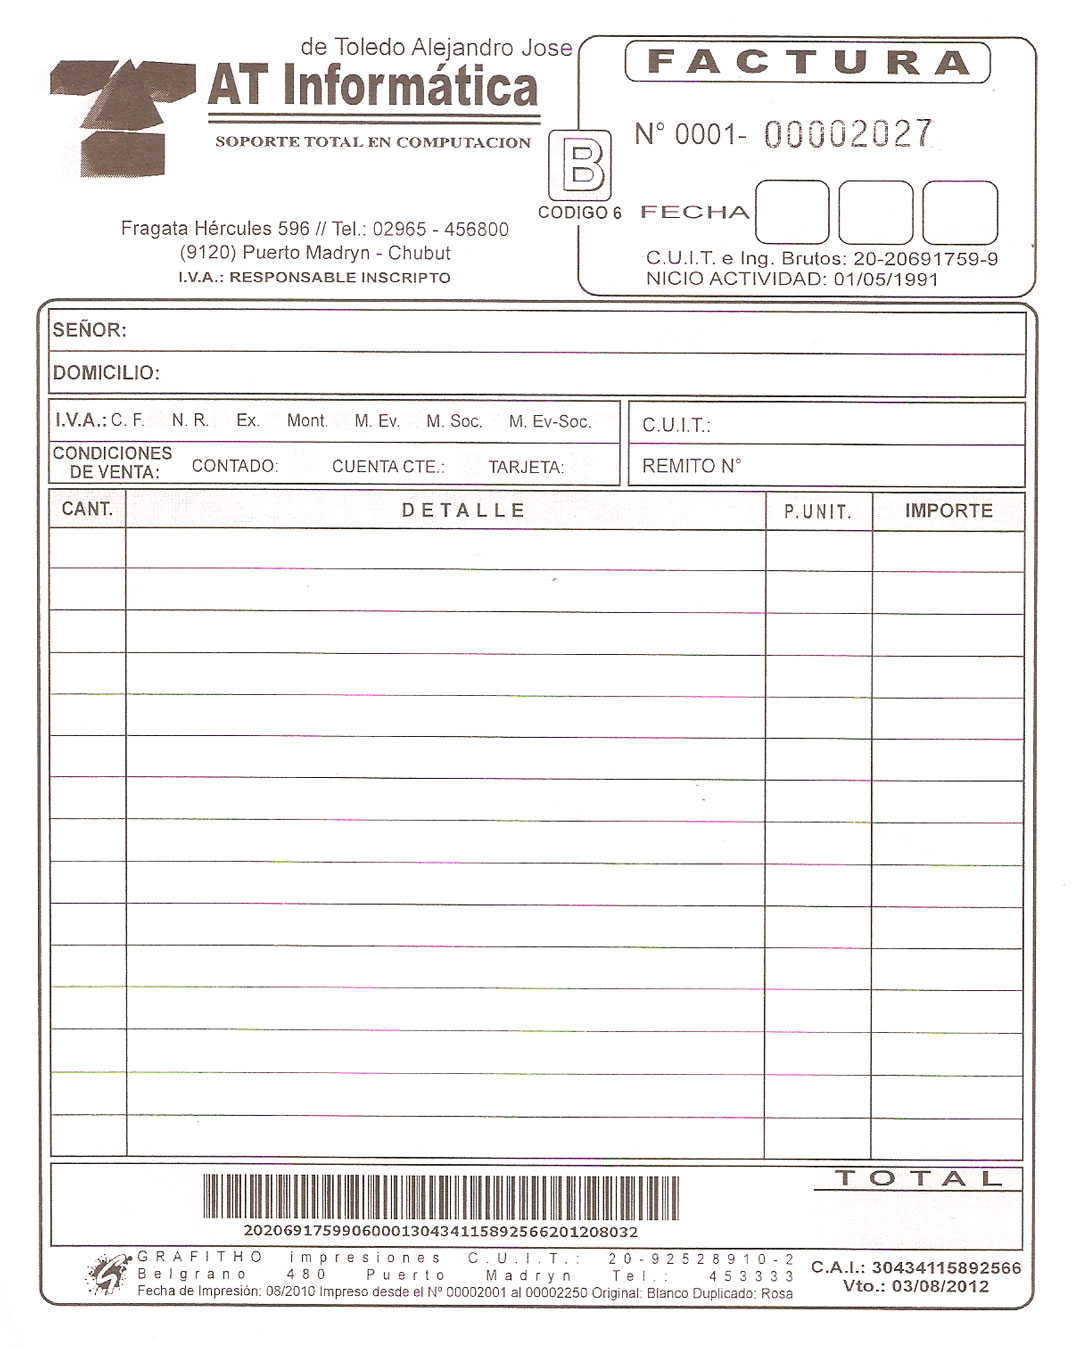
\includegraphics[scale=0.3]{images/atinformatica-facturaB.jpg}
    \caption{Factura}
    \end{figure}

    \begin{figure}[h]
    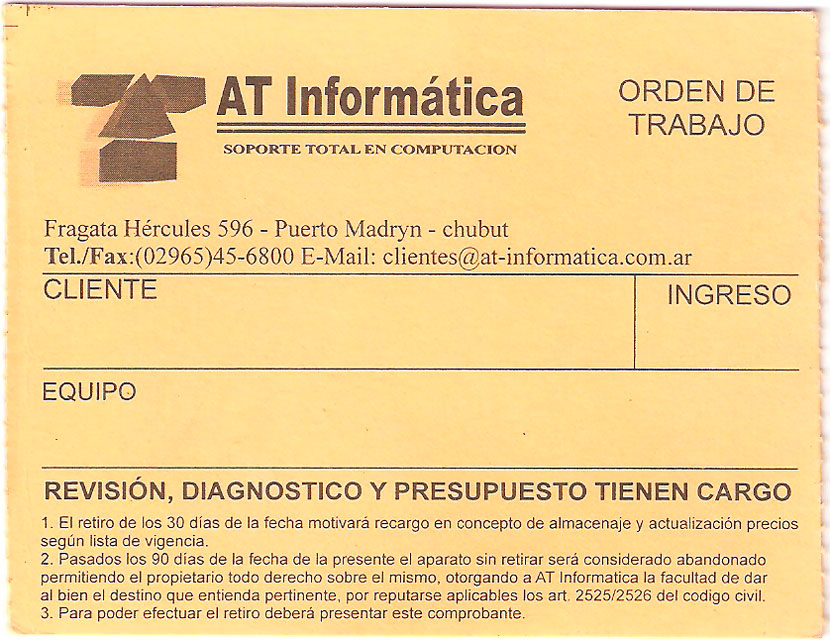
\includegraphics[scale=0.5]{images/atinformatica-orden_de_trabajo.jpg}
    \caption{Orden de trabajo}
    \end{figure}

    \begin{figure}[h]
    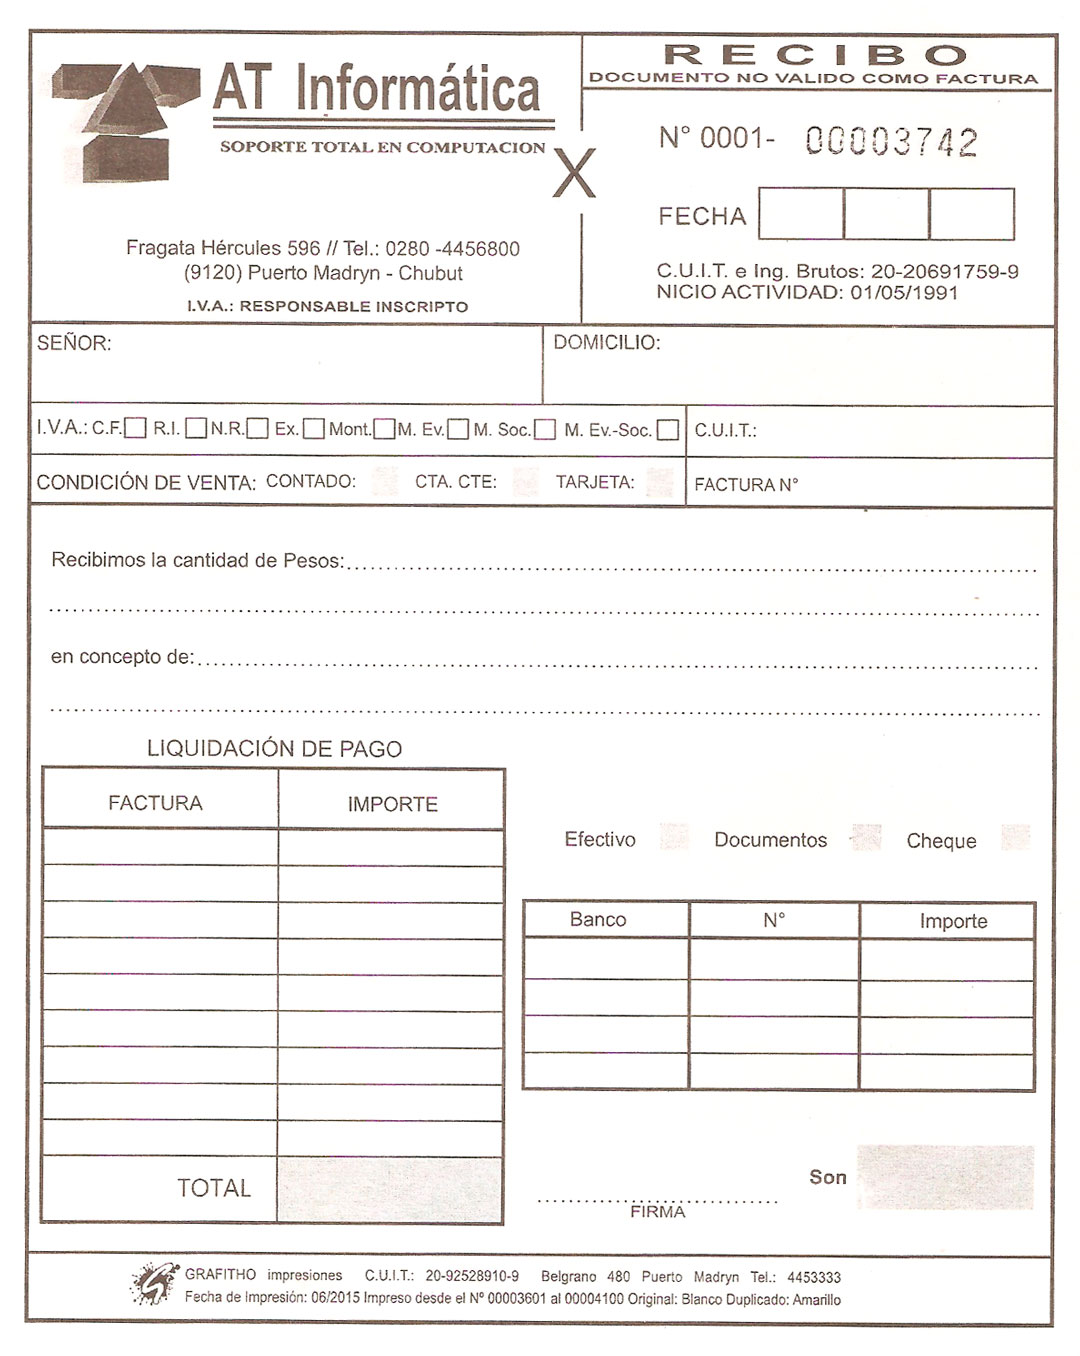
\includegraphics[scale=0.4]{images/atinformatica-recibo.jpg}
    \caption{Recibo}
    \end{figure}

    \begin{figure}[h]
    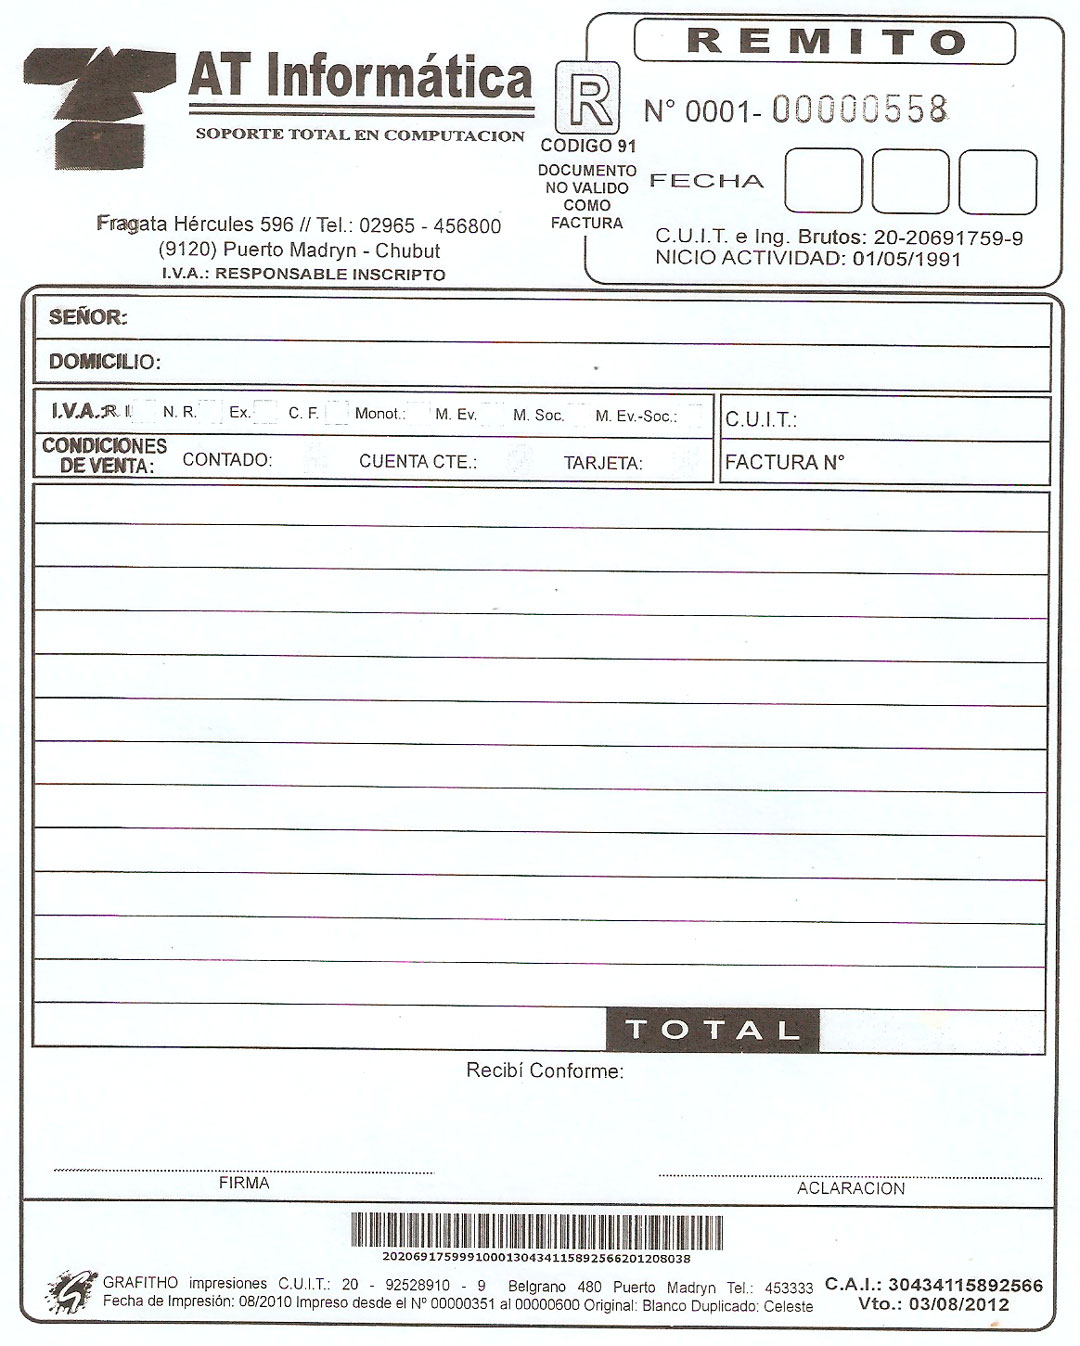
\includegraphics[scale=0.4]{images/atinformatica-remito.jpg}
    \caption{Remito}
    \end{figure}

    \begin{figure}[h]
    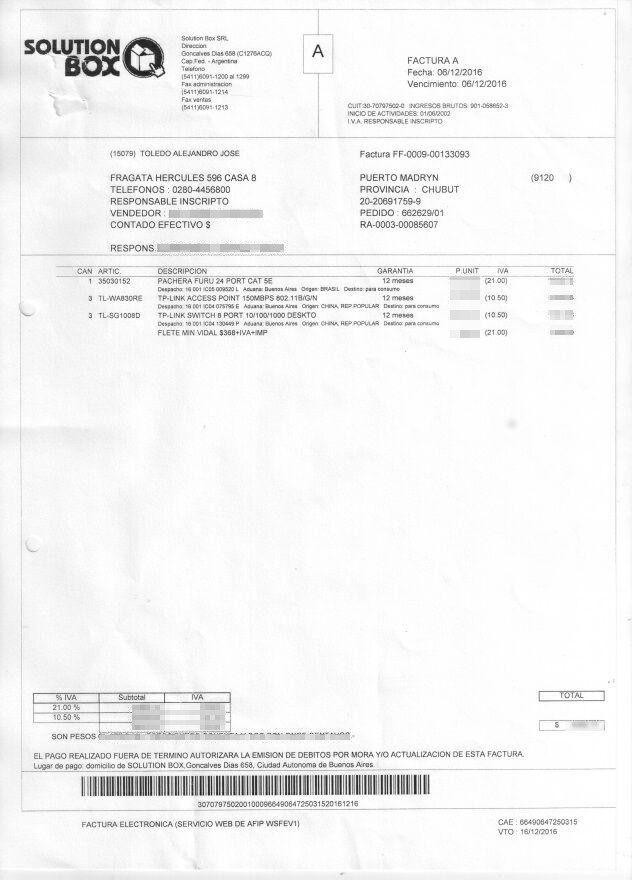
\includegraphics[scale=0.4]{images/atinformatica-remito1.jpg}
        \caption{Remito (proveedor)}
    \end{figure}

    \begin{figure}[h]
    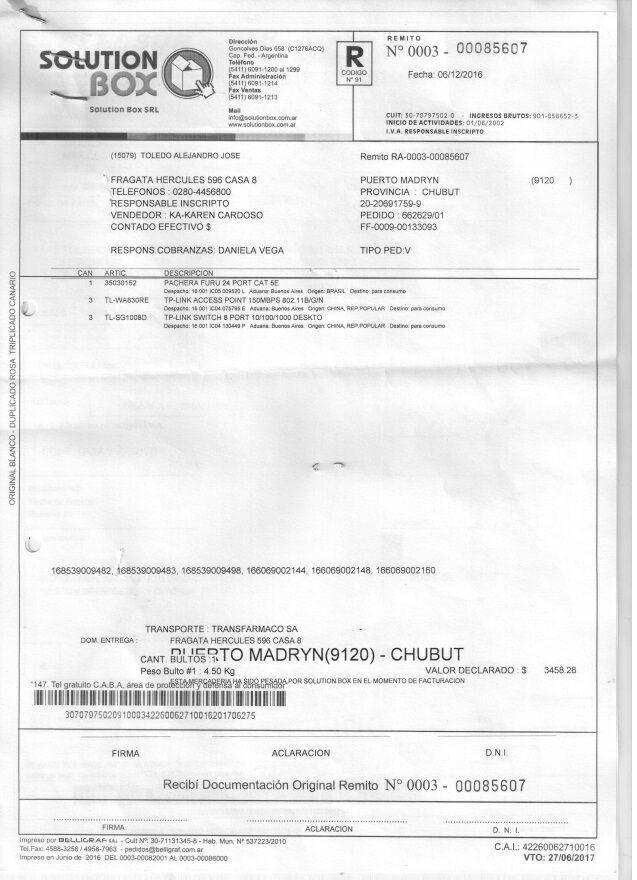
\includegraphics[scale=0.4]{images/atinformatica-remito2.jpg}
        \caption{Remito (proveedor)}
    \end{figure}

    \begin{figure}[h]
    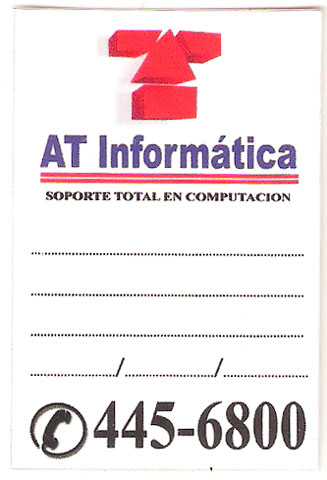
\includegraphics[scale=0.275]{images/atinformatica-sticker.jpg}
    \caption{Sticker}
    \end{figure}

    \begin{figure}[h]
    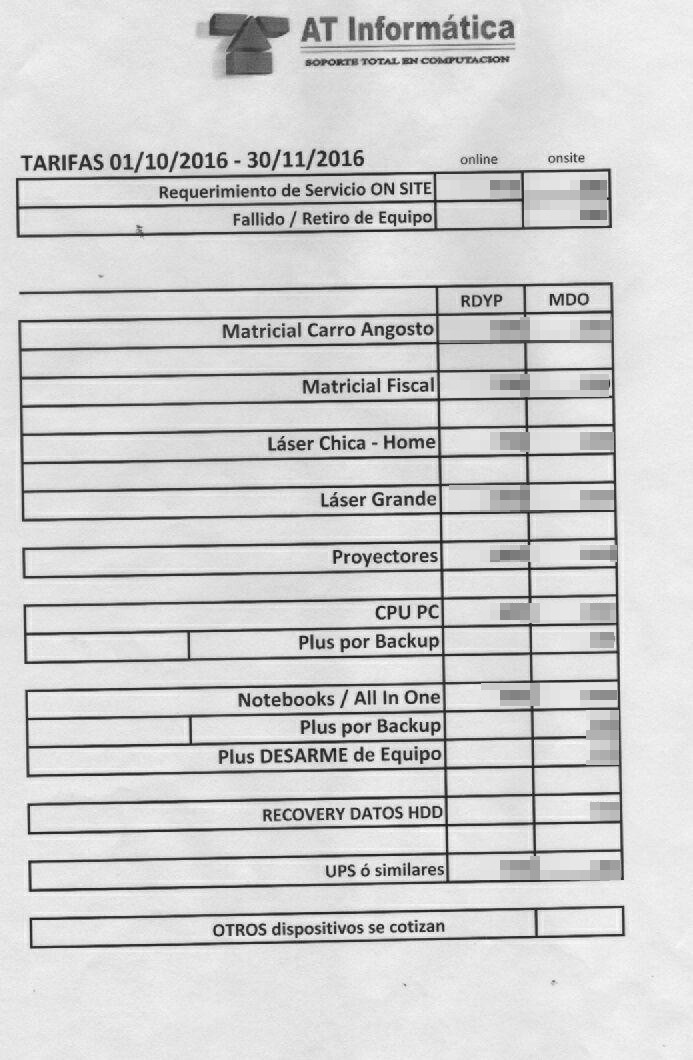
\includegraphics[scale=0.5]{images/atinformatica-tarifario-pixel.jpg}
    \caption{Tarifario}
    \end{figure}

    \begin{figure}[h]
    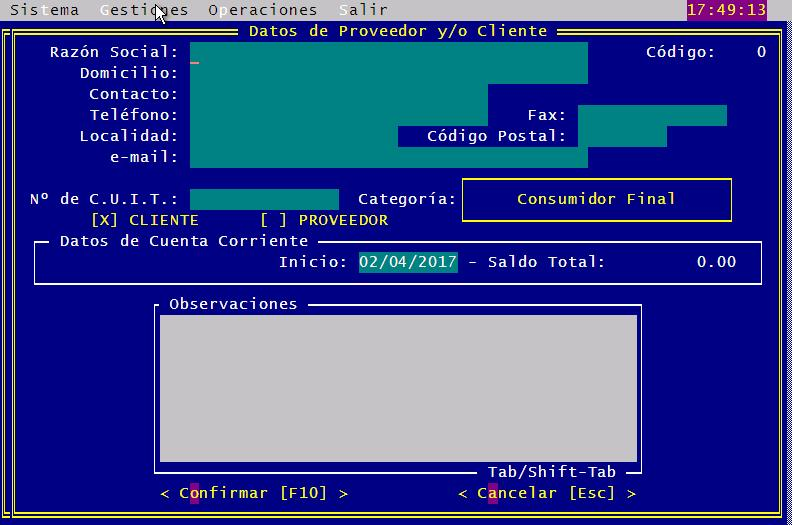
\includegraphics[scale=0.5]{images/cliente_ingreso.jpg}
    \caption{Factura}
    \end{figure}

    \begin{figure}[h]
    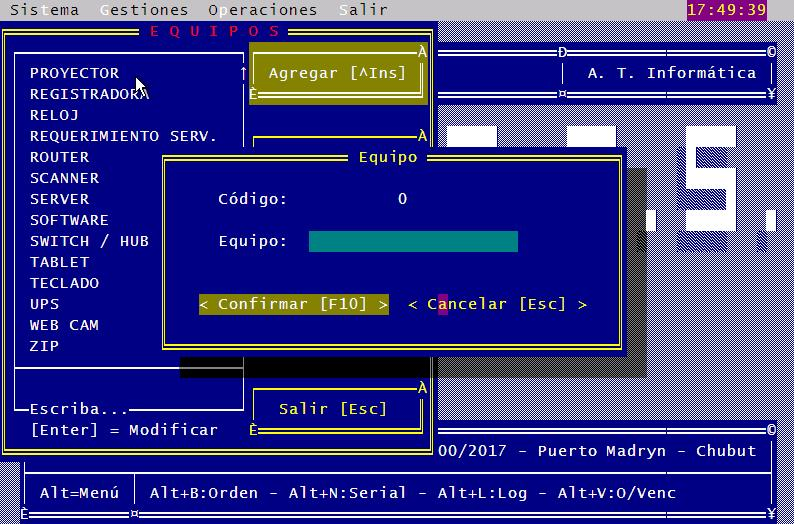
\includegraphics[scale=0.5]{images/equipo_e_ingreso.jpg}
    \caption{Listado de equipos e ingreso}
    \end{figure}

    \begin{figure}[h]
    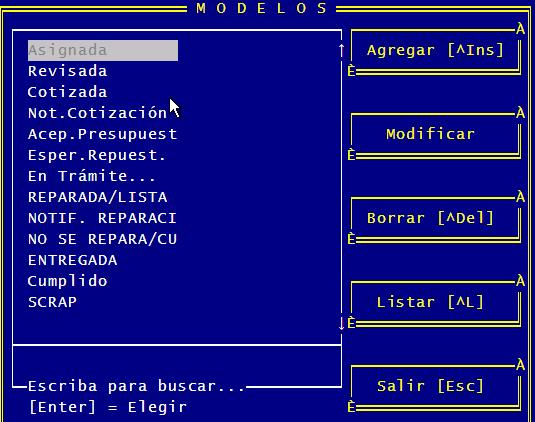
\includegraphics[scale=0.5]{images/estados_orden.jpg}
    \caption{Estados de una orden}
    \end{figure}

    \begin{figure}[h]
    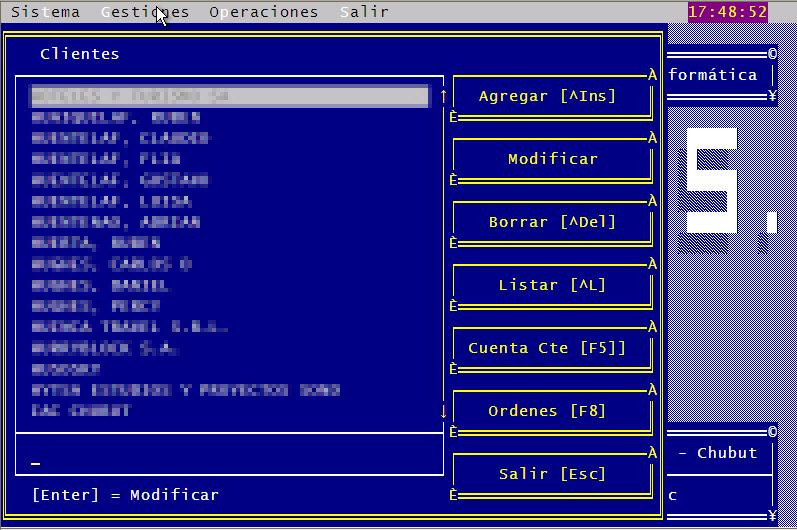
\includegraphics[scale=0.5]{images/listado_clientes.jpg}
    \caption{Listado de clientes}
    \end{figure}

    \begin{figure}[h]
    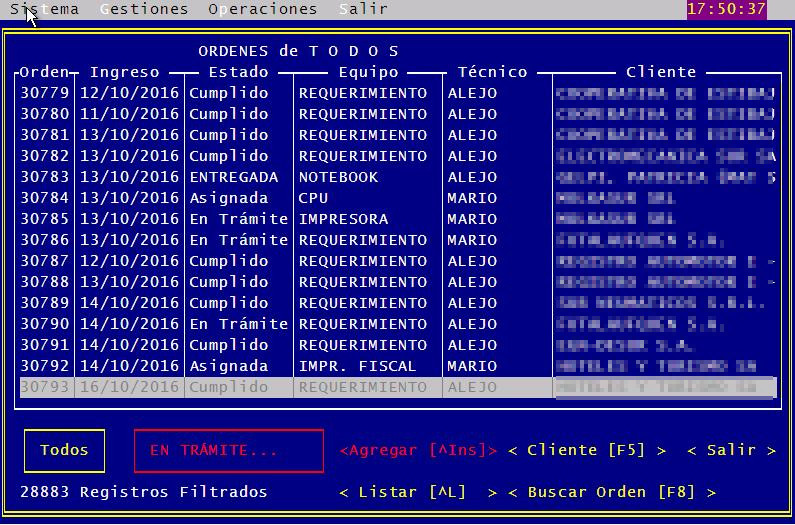
\includegraphics[scale=0.5]{images/listado_ordenes.jpg}
    \caption{Listado de órdenes}
    \end{figure}

    \begin{figure}[h]
    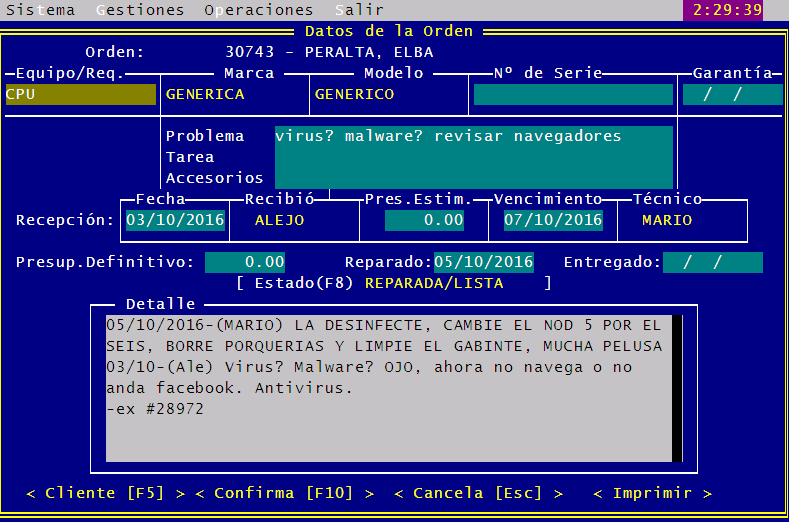
\includegraphics[scale=0.5]{images/orden1.png}
    \caption{Orden de trabajo}
    \end{figure}

    \begin{figure}[h]
    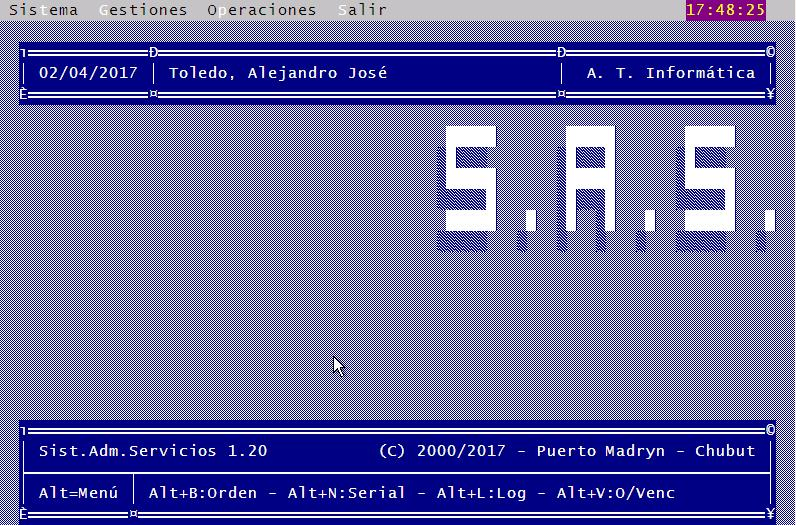
\includegraphics[scale=0.5]{images/pantalla_principal.jpg}
    \caption{Pantalla principal}
    \end{figure}

\clearpage

\section{Anexo 2 - Estados de las Órdenes de Trabajo}

    \begin{enumerate}
        \item \textbf{Asignada}: estado inicial de la orden. Cuenta con un técnico asociado.
        \item \textbf{Revisada}: el técnico asociado realizó un primer diagnóstico del equipo ingresado (se lo anexa a la OT; incluye el problema que describió el cliente y lo que descubrió el técnico).
        \item \textbf{Cotizada}: equipo ya diagnosticado. Presupuesto elaborado.
        \item \textbf{Notificada de cotización}: el cliente ya fue notificado del presupuesto. En caso de que el cliente no acepte, la orden pasa al estado \textbf{No se repara} o bien a \textbf{Fallida} (en caso de tratarse de una visita). 
        \item \textbf{Presupuesto aceptado}: el cliente aceptó el presupuesto indicado para realizar el trabajo.
        \item \textbf{Espera de repuestos}: se pidieron repuestos necesarios para realizar el trabajo. No se puede reanudar hasta su arribo.
        \item \textbf{En trámite}: se está realizando el trabajo; durante esta etapa, varios técnicos pueden participar en el trabajo y realizar observaciones en la orden. En caso de que el trabajo requiera algún servicio más, la OT vuelve a pasar por los estados \textbf{Cotizada}, \textbf{Notificada de cotización}, y en caso de aceptarse el presupuesto, \textbf{Presupuesto aceptado}. En caso de no aceptarse, se pasa a \textbf{No se repara} o a \textbf{Fallida} (si es una visita).
        \item \textbf{Pendiente de facturación}: trabajo terminado. 
        \item \textbf{Notificada de reparación}: se le avisa al cliente que su equipo está listo para ser retirado.
        \item \textbf{Cumplido}: se realizó la visita exitosamente. La orden se encuentra pendiente de facturación.
        \item \textbf{No se repara}: no se completó la reparación porque el cliente no aceptó el presupuesto.
        \item \textbf{Fallida}: no se pudo completar el trabajo on-site.
        \item \textbf{Entregada}: se entregó el equipo reparado al cliente. El trabajo fue facturado.
        \item \textbf{SCRAP}: el cliente no retiró el equipo pasados los 60 (sesenta) días hábiles. Se encuentra a disposición de la organización.
    \end{enumerate}

\end{document}
